\documentclass[master=emitm,masteroption=bc,oneside]{kulemt}
\DisemulatePackage{setspace}
\usepackage{setspace}
\usepackage{pdfpages}
\usepackage{amsmath}
\usepackage{pgf,tikz}
\usepackage{mdframed}
\usepackage{float}
\usepackage{tabularx}
\usepackage{listings}
%\usepackage[utf8]{inputenc}
\usetikzlibrary{positioning, arrows.meta, matrix, backgrounds, shapes.misc}
\usetikzlibrary{calc,arrows}
\usepackage{verbatim}
\usepackage[left=1cm,right=1cm]{geometry}
%\pagestyle{empty}
\usetikzlibrary{shapes.geometric}
\usepackage{mathptmx}
\usepackage[10pt]{moresize}
\usepackage[acronym]{glossaries}




\makeatletter

%%%%%%%%%%%%%%%%%%% Begin add-int-rnd %%%%%%%%%%%%%%%
% Data Flip Flip (DFF) shape
\pgfdeclareshape{dff}{
	% The 'minimum width' and 'minimum height' keys, not the content, determine
	% the size
	\savedanchor\northeast{%
		\pgfmathsetlength\pgf@x{\pgfshapeminwidth}%
		\pgfmathsetlength\pgf@y{\pgfshapeminheight}%
		\pgf@x=0.5\pgf@x
		\pgf@y=0.5\pgf@y
	}
	% This is redundant, but makes some things easier:
	\savedanchor\southwest{%
		\pgfmathsetlength\pgf@x{\pgfshapeminwidth}%
		\pgfmathsetlength\pgf@y{\pgfshapeminheight}%
		\pgf@x=-0.5\pgf@x
		\pgf@y=-0.5\pgf@y
	}
	% Inherit from rectangle
	\inheritanchorborder[from=rectangle]
	
	% Define same anchor a normal rectangle has
	\anchor{center}{\pgfpointorigin}
	\anchor{north}{\northeast \pgf@x=0pt}
	\anchor{east}{\northeast \pgf@y=0pt}
	\anchor{south}{\southwest \pgf@x=0pt}
	\anchor{west}{\southwest \pgf@y=0pt}
	\anchor{north east}{\northeast}
	\anchor{north west}{\northeast \pgf@x=-\pgf@x}
	\anchor{south west}{\southwest}
	\anchor{south east}{\southwest \pgf@x=-\pgf@x}
	\anchor{text}{
		\pgfpointorigin
		\advance\pgf@x by -.5\wd\pgfnodeparttextbox%
		\advance\pgf@y by -.5\ht\pgfnodeparttextbox%
		\advance\pgf@y by +.5\dp\pgfnodeparttextbox%
	}
	
	% Define anchors for signal ports
	\anchor{D}{
		\pgf@process{\northeast}%
		\pgf@x=-1\pgf@x%
		\pgf@y=.5\pgf@y%
	}
	\anchor{CLK}{
		\pgf@process{\northeast}%
		\pgf@x=-1\pgf@x%
		\pgf@y=-.66666\pgf@y%
	}
	\anchor{CE}{
		\pgf@process{\northeast}%
		\pgf@x=-1\pgf@x%
		\pgf@y=-0.33333\pgf@y%
	}
	\anchor{Q}{
		\pgf@process{\northeast}%
		\pgf@y=.5\pgf@y%
	}
	\anchor{Qn}{
		\pgf@process{\northeast}%
		\pgf@y=-.5\pgf@y%
	}
	\anchor{R}{
		\pgf@process{\northeast}%
		\pgf@x=0pt%
	}
	\anchor{S}{
		\pgf@process{\northeast}%
		\pgf@x=0pt%
		\pgf@y=-\pgf@y%
	}
	% Draw the rectangle box and the port labels
	\backgroundpath{
		% Rectangle box
		\pgfpathrectanglecorners{\southwest}{\northeast}
		% Angle (>) for clock input
		\pgf@anchor@dff@CLK
		\pgf@xa=\pgf@x \pgf@ya=\pgf@y
		\pgf@xb=\pgf@x \pgf@yb=\pgf@y
		\pgf@xc=\pgf@x \pgf@yc=\pgf@y
		\pgfmathsetlength\pgf@x{1.6ex} % size depends on font size
		\advance\pgf@ya by \pgf@x
		\advance\pgf@xb by \pgf@x
		\advance\pgf@yc by -\pgf@x
		\pgfpathmoveto{\pgfpoint{\pgf@xa}{\pgf@ya}}
		%		\pgfpathlineto{\pgfpoint{\pgf@xb}{\pgf@yb}}
		%		\pgfpathlineto{\pgfpoint{\pgf@xc}{\pgf@yc}}
		\pgfclosepath
		
		% Draw port labels
		\begingroup
		\tikzset{flip flop/port labels} % Use font from this style
		\tikz@textfont
		\endgroup
	}
}

%%%%%%%%%%%%%%%%%%% End add-int-rnd %%%%%%%%%%%%%%%

% Key to add font macros to the current font
\tikzset{add font/.code={\expandafter\def\expandafter\tikz@textfont\expandafter{\tikz@textfont#1}}} 

% Define default style for this node
\tikzset{flip flop/port labels/.style={font=\sffamily\scriptsize}}
\tikzset{every dff node/.style={draw,minimum width=1.0cm,minimum 
		height=0.5cm,very thick,inner sep=1mm,outer sep=0pt,cap=round,add 
		font=\sffamily}}
%\usepackage{kulemtx}
%\headstyles{kulemtman}
%\kulemtmanToC


\setup{title={Metrics of Operating System Security Components in Virtual Environments},
  author={Oliver Jessl},
  promotor={Prof. Dr.-Ing. Clemens Martin},
  assessor={Prof. Dr.-Ing. habil. Dennis Pfisterer},
  assistant={}}
% The following \setup may be removed entirely if no filing card is wanted
\setup{filingcard,
  translatedtitle=,
  udc=621.3,
  shortabstract={Here comes a very short abstract, containing no more than 500
    words. \LaTeX\ commands can be used here. Blank lines (or the command
    \texttt{\string\pa r}) are not allowed!
    \endgraf \lipsum[2]}}
% Uncomment the next line for generating the cover page
%\setup{coverpageonly}
% Uncomment the next \setup to generate only the first pages (e.g., if you
% are a Word user.
%\setup{frontpagesonly}

\setlrmarginsandblock{3cm}{3cm}{*}
\setulmarginsandblock{3cm}{3cm}{*}
\checkandfixthelayout

% Choose the main text font (e.g., Latin Modern)
\setup{font=times}

% If you want to include other LaTeX packages, do it here. 

% Finally the hyperref package is used for pdf files.
% This can be commented out for printed versions.
\usepackage[pdfusetitle,colorlinks,plainpages=false]{hyperref}

%%%%%%%
% The lipsum package is used to generate random text.
% You never need this in a real master's thesis text!
\IfFileExists{lipsum.sty}%
 {\usepackage{lipsum}\setlipsumdefault{11-13}}%
 {\newcommand{\lipsum}[1][11-13]{\par And some text: lipsum ##1.\par}}
%%%%%%%



%\onehalfspacing
\onehalfspacing

\include{glossary.tex}

\makeglossaries

%\includeonly{chap-n}
\begin{document}


\tableofcontents*

\begin{abstract}
  The \texttt{abstract} environment contains a more extensive overview of
  the work. But it should be limited to one page.

  \lipsum[1]
\end{abstract}

% A list of figures and tables is optional
%\listoffigures
%\listoftables
% If you only have a few figures and tables you can use the following instead
\listoffiguresandtables
% The list of symbols is also optional.
% This list must be created manually, e.g., as follows:
\chapter{List of Abbreviations and Symbols}
\section*{Abbreviations}
\begin{flushleft}
  \renewcommand{\arraystretch}{1.1}
  \begin{tabularx}{\textwidth}{@{}p{12mm}X@{}}
    ASLR  & Address Space Randomization Layout \\  	
    GRI   & Get Random Int (Random Number Generator)\\
	GRL	  & Get Random Long (Random Number Generator)\\
	IRQ	  & Interrupt Request \\
	LTS	  & Long Term Support\\
    NIST  & National Institute of Standards and Technology \\
    PRNG  & Pseudo Random Number Generator \\    
	TLS   & Transport Socket Layer \\           
    TRNG  & True Random Number Generator \\ 
    VM	  & Virtual Machine \\
  \end{tabularx}
\end{flushleft}
\section*{Symbols}
\begin{flushleft}
  \renewcommand{\arraystretch}{1.1}
  \begin{tabularx}{\textwidth}{@{}p{12mm}X@{}}
    42    & ``The Answer to the Ultimate Question of Life, the Universe,
            and Everything'' according to \cite{h2g2} \\
    $c$   & Speed of light \\
    $E$   & Energy \\
    $m$   & Mass \\
    $\pi$ & The number pi \\
  \end{tabularx}
\end{flushleft}


% Now comes the main text
\mainmatter

\chapter{Introduction}
\label{cha:intro}
\section{Motivation}
Operating systems implement a variety of security components which depend significantly on the entropy of random numbers. In general, those random numbers can be provided by operating system internal or external providers, so called Random Number Generators (RNG). Typical external providers are hardware devices, able to deviate random numbers from radioactive decay, atmospheric or thermal noise, photoelectric effects etc. Since those numbers are assumed to provide a high level of entropy i.e. random numbers of high quality, they are also referred as True Random Number Generators (TRNG). Contrary, RNGs implemented as part of an operating system, the lack of comparable stochastic processes and hence are labeled as Pseudo Random Number Generator (PRNG). To compensate this lack, PRGN implementations need to fall back on alternative sources, able to provide information with a certain degree of entropy. Common approaches of operating systems usually adopt information from external sources, f.e. user input like keyboard events or mouse coordinates. Beside further external input like network traffic, system internal individual information like serial numbers of hardware devices, MAC addresses or the occurrence of hardware interrupts is used to gain an entropy pool of pseudo random numbers. Consequently, the process of generating random numbers by an operating system PRNG is influenced by the way the system interacts with its environment i.e. how it is set up. This aspect should be considered when applying server operating systems as virtual machines i.e. in virtual environments. \\~\\
Virtualization of operating systems has increased continuously over the recent years and layed the foundations for new resource management concepts and business models like f.e. cloud hosting. Regarding server virtualization, many organizations exceed rates of 75\% \cite{gartnervmmarket}. By executing an operating system as a virtual machine, improvements in several areas, like scalability and more efficient utilization of hardware resources, backup \& disaster recovery strategy, accelerated provision of new system instances etc. can be achieved. Depending on the applied technology, such virtual machines can be setup up on basis of operating system setup images which are targeted for installation directly on hardware, without any further modification required. In other words, the virtual machine monitor or hypervisor enables the execution of regular commercial or open source operating systems in a virtual environment. However, while there are many reasons to utilize virtual machines, most of the standard security practices of operating systems are based on assumptions that hold true for physical machines, but don't translate immediately into the domain of virtualized machines \cite{kerrigan2012study}. A virtual hosted Linux server f.e. will never receive a user triggered event during the boot process, which is a critical period within the initialization of the internal Linux PRNG. Further, new virtual machine instances are usually provided by cloning a master image, instead of running an installation setup, leading to a higher degree of homogeneity among virtual machine instances. While provisioning time and maintenance benefit from this practice, it may be regarded critical. If this approach f.e. is applied as the standard process of a cloud hosting provider, it`s customers may be delivered a vulnerable system from the outset, since one customer might gain insights regarding another customers system, just by analyzing his own. These insights can be used to exploit VM reset vulnerabilities which take advantage of the reuse of  operating system snapshots, so called snapshot replay. Thomas Ristenpart et. al. describe this type of attack and apply it on TSL implementations with disastrous results. Relevant reasons they identified are the exposure of randomness, as well as the inability to find sufficient entropy in virtual systems environments \cite{ristenpart2010good, ristenpart2009hey}. \\~\\
According to a study of Gartner from 2016, the market for x86 server virtualization infrastructure software is partitioned among few competitors, led by VMWare, Microsoft, Oracle and Red Hat. While VMWare and Microsoft offer proprietary solutions, Oracle and Red Hat adopted the open-source Xen-hypervisor technology. For cloud infrastructures, the Xen-hypervisor remains the most widely used architecture for public infrastructure as a service (IaaS) cloud provider. This fact is predominantly attributable to Amazon's utilization of the Xen-hypervisor for its cloud solutions "Amazon Web Services" \cite{bittman2016magic}. Similarly, the market of common server operating systems can be divided into proprietary and open-source solutions. While Microsoft dominates the fraction of proprietary systems with its Windows Server series, Linux based systems have a total share of \~37\%. Within this share, \~39\% of servers dedicated to host websites etc. are running an Ubuntu Distribution \cite{statsharelinux} . \\~\\
Summarized, recent studies have revealed that virtualization of Linux based servers is widespread, while the execution of those systems as virtual machine may bring up critical vulnerabilities. Based on these considerations the objective of this thesis is an analysis of the generation of random numbers by a Linux 4.X.X.X kernel's internal PRNG in a Xen-hypervisor environment. To this date, several research contributions have been published in this field. Those may be divided by their scope regarding the Linux PRNG responsibilities, attack vectors and, if analyzing the entropy pools state, the approach of assessing randomness. While some papers address the PRNG output for the entire time of a system's uptime, the focus of this research will be a system's startup i.e. boot phase. This period is meant to be of certain interest for several reasons: The initialization of the Linux PRMG is beginning as one of the first activities conducted when a (virtual) machine starts to bring up the systems kernel, as it is eager to use as many noise sources as possible to build up various entropy pools. Further, during this initialization process, some buffers are assigned with values which are valid and reused over the entire uptime of the system. Poorly developed values for these buffers are assumed to weaken a number of security components and hence are of particular interest. Finally, a part of the boot process is the startup of various daemon processes, which usually remain in execution over the entire system uptime. Beside daemons required by the system, this may also be applications like web-, ftp-, ssh-, proxy-servers which may be reachable via the internet and thus potentially vulnerabilities should be classified as critical.
To obtain a comprehensive data record for evaluation, a Linux 4.X.X.X kernel has been enhanced by a tracking feature, able to record information at points of interest, without producing any noise itself. The feature is not just able to track the values returned to applications requesting random values, but also to breakdown how those have been generated over several stages until their origin in terms of noise. This kernel is brought up within an Ubuntu Server 16.04 system, hosted as a guest on Xen hypervisor 4.XX. The Linux PRNG has an internal rating system describing an entropy pools quality in "bits of entropy". Some research contributions (f.e. \cite{lacharme2012linux})refer to this system when assessing random number quality. To conduct an independent and fine grained analysis, for this thesis a Statistical Test Suite, published by the NIST has been applied \cite{paul2016nist}. Various operating systems security concepts rely on solid random numbers. Hence, besides the processing of noise to random numbers, also the consequences of weak random numbers have been analyzed on the effectiveness of two fundamental operating system security technologies: Stack Guards/Stack Canaries and Address Space Randomization Layout (ASLR).
The following sections will deliver the required background knowledge regarding virtualization via the Xen-hyperisor, the architecture and generation of the Linux Pseudo Random Number Generator, the concepts of stack canaries and ASLR and Statistical Random Number Validation. 



\section{Related Reserach}

Xen

----------------

ASLR

----------------

XEN/PRNG

If the correlation between the jiffies counter J and the cycle counter CC is known (they are based on the same underlying clock), then the only unknown to an attacker is CC at the time each output is generated. \cite{everspaugh2014not} VMWare beginnt mit CC=0 => katastrophal \cite{everspaugh2014not} Seite 8. Dort ansetzten, ist es bei Xen ebenso?

----------------











% Virtualization in these terms means, that an operating system is not directly installed on a hardware host. Instead on the host machine an application is installed beeing able administer systems resources and assign those to several operating systems which may be run on host simultaneously.  

   





%%% Local Variables: 
%%% mode: latex
%%% TeX-master: "thesis"
%%% End: 

\chapter{The First Chapter}
\label{cha:1}
The following section will deliver the relevant information regarding memory management an ASLR.

% EVP (Enhanced Virus Protection) – available on
all 64-bit AMD CPUs (starting in 2003)
\cite{guide2017amd64}

% XD Bit (Execute Disable Bit) – available with
Pentium 4 "Prescott" core (starting in 2004)1
\cite{guide2017intel}
If the execute-disable bit of a memory page is set, that page can be used only as data. An attempt to execute code
from a memory page with the execute-disable bit set causes a page-fault exception.

\section{Memory Management}
Modern Operation System implement an abstraction layer.

Load elf: sections -> segments.
-------------------------------------------
Virtual Address space (linearer Adressraum)
--------------------------------------------
Linear Address Space
From a user perspective, the address space is a at linear address space but pre-
dictably, the kernel's perspective is very different. The address space is split into
two parts, the userspace part which potentially changes with each full context switch
and the kernel address space which remains constant. The location of the split is
determined by the value of PAGE\_OFFSET which is at 0xC0000000 on the x86. This
means that 3GiB is available for the process to use while the remaining 1GiB is
always mapped by the kernel. The linear virtual address space as the kernel sees it
is illustrated in Figure 4.1.
\cite{gorman2004linuxvmmgr}


Up Down Kernel/User space
--------------------------












\cite{cowan2000buffer}
\cite{marco2014effectiveness}
\cite{kerrigan2012study}
\cite{guide2017intel}
\cite{wojtczuk2011following}
\cite{alt2015entropy}
\cite{thompsonrandomness}
\cite{celesti2010improving}
\cite{mueller@bsi1}
\cite{mueller@bsi2}
\cite{marco2013preventing}


%\section{The First Topic of the Chapter}
%First comes the introduction to this topic.
%
%\lipsum[55]
%
%\subsection{An item}
%Please don't abuse enumerations: short enumerations shouldn't use
%``\verb|itemize|'' or ``\texttt{enumerate}'' environments.
%So \emph{never write}: 
%\begin{quote}
%  The Eiffel tower has three floors:
%  \begin{itemize}
%  \item the first one;
%  \item the second one;
%  \item the third one.
%  \end{itemize}
%\end{quote}
%But write:
%\begin{quote}
%  The Eiffel tower has three floors: the first one, the second one, and the
%  third one.
%\end{quote}
%
%\section{A Second Topic}
%\lipsum[64]
%
%\subsection{Another item}
%\lipsum[56-57]
%
%\section{Conclusion}
%The final section of the chapter gives an overview of the important results
%of this chapter. This implies that the introductory chapter and the
%concluding chapter don't need a conclusion.
%
%\lipsum[66]

%%% Local Variables: 
%%% mode: latex
%%% TeX-master: "thesis"
%%% End: 

\chapter{The Next Chapter}
\label{cha:2}

\section{Operating System Virtualization with the Xen-Hypervisor}

Virtualization of operating systems has increased continuously over the recent years and layed the foundations for new resource management concepts and business models like f.e. cloud hosting. Regarding server virtualization, many organizations exceed rates of 75\% \cite{gartnervmmarket}. By executing an operating system as a virtual machine (VM), improvements in several areas can be achieved. As instances of even different operating systems can be run parallel on the same host machine, system capacity in terms of processing power, volatile and persistent memory can be utilized more efficient. A VM can even be assigned resources dynamically at runtime, without the need of a restart. Further, backup \& recovery strategies can be simplified, as a VM's physical presentation at any certain state can be preserved in files. This even enables to move a running VM from one to another server in the same resource pool with virtually no service interruption \cite{migratevms}. Also the process of providing a new VM instance can be slimmed down drastically. Instead of being required to execute an operating system setup for a particular hardware composition, a once created VM master image can be cloned and configured. Depending on the applied technology, VMs can be setup up on basis of operating system setup images which are targeted for installation directly on hardware, without any further modification required. In other words, the virtual machine monitor or hypervisor enables the execution of regular proprietary or open source operating systems in a virtual environment. \\
According to a study of Gartner from 2016, the market for x86 server virtualization infrastructure software is partitioned among few competitors, led by VMWare, Microsoft, Oracle and Red Hat. While VMWare and Microsoft offer proprietary solutions, Oracle and Red Hat adopted the open-source Xen-hypervisor technology. For cloud infrastructures, the Xen-Hypervisor remains the most widely used architecture for public infrastructure as a service (IaaS) cloud provider. This fact is predominantly attributable to Amazon's utilization of the Xen-Hypervisor for its cloud solutions "Amazon Web Services" \cite{bittman2016magic}.
\\~\\
Hier muss noch ein Uebergang hin
\\


- Open Source
- Amazon
- Verbreitung 
- HVM / PVM
- Architektur

------------------------------------
\cite{everspaugh2014not}
Second,aVM  can be repeatedly executed froma ?xed image which is the default for amazon
Dort auch: infos zu regualr boot/snapshot/masterimage
------------------------------------



However, while there are many reasons to utilize virtual machines, most of the standard security practices of operating systems are based on assumptions that hold true for physical machines, but don't translate immediately into the domain of virtualized machines \cite{kerrigan2012study}. A virtual hosted Linux server f.e. will never receive a user triggered event during the boot process, which is a critical period within the initialization of the internal Linux PRNG. Further, new virtual machine instances are usually provided by cloning a master image, instead of running an installation setup, leading to a higher degree of homogeneity among virtual machine instances. While provisioning time and maintenance benefit from this practice, it may be regarded critical. If this approach f.e. is applied as the standard process of a cloud hosting provider, it`s customers may be delivered a vulnerable system from the outset, since one customer might gain insights regarding another customers system, just by analyzing his own. These insights can be used to exploit VM reset vulnerabilities which take advantage of the reuse of  operating system snapshots, so called snapshot replay. Thomas Ristenpart et. al. describe this type of attack and apply it on TSL implementations with disastrous results. Relevant reasons they identified are the exposure of randomness, as well as the inability to find sufficient entropy in virtual systems environments \cite{ristenpart2010good, ristenpart2009hey}. \\~\\
According to a study of Gartner from 2016, the market for x86 server virtualization infrastructure software is partitioned among few competitors, led by VMWare, Microsoft, Oracle and Red Hat. While VMWare and Microsoft offer proprietary solutions, Oracle and Red Hat adopted the open-source Xen-hypervisor technology. For cloud infrastructures, the Xen-hypervisor remains the most widely used architecture for public infrastructure as a service (IaaS) cloud provider. This fact is predominantly attributable to Amazon's utilization of the Xen-hypervisor for its cloud solutions "Amazon Web Services" \cite{bittman2016magic}. 

Similarly, the market of common server operating systems can be divided into proprietary and open-source solutions. While Microsoft dominates the fraction of proprietary systems with its Windows Server series, Linux based systems have a total share of \~37\%. Within this share, \~39\% of servers dedicated to host websites etc. are running an Ubuntu Distribution \cite{statsharelinux} . \\~\\


\section{Random Number Generation in Linux x64 Kernel 4.4}

\subsection{General}

Random numbers are required by a variety of security related applications. An obvious purpose is encryption or signing of data, like f.e. disk encryption, Transport Socket Layer (TLS) or digital signatures of emails. In this case random numbers are used to generate cryptographically secure keys. Concepts like Stack Canaries (aka. Stack Guards) or Address Space Layout Randomization (ASLR) rely purely on the nondeterministic character of random numbers, applying them to make certain types of attacks on vulnerable applications much more difficult. Overall, the effectiveness of such applications depends significantly on the quality i.e. unpredictably of random numbers, provided by an operating system. \\
In the following a comprehensive introduction to the Linux Random Number Generator (LRNG) with focus on analyzed concepts and components of this thesis will be given. It refers to Linux kernel v.4.4, which is currently used in several major Long Term Support distributions like Ubuntu Server 16.04 LTS. If facts are valid for Intel x86/x64 platforms only, those will be noted as such.\\
In general, many modern CPU-architectures implement an on-chip True Random Number Generator \cite{guide2017intel}. Starting with 'IvyBridge' architecture, Intel provides two instructions accessing directly those entropy sources. The \textsf{RDRAND} instruction returns random numbers that are supplied by a cryptographically secure, deterministic random bit generator (DRBG). The DRBG is designed to meet the NIST SP 800-90A standard. If an application or operating system design insists on applying in it's own Pseudo Random Number Generator (PRNG) it may apply the \textsf{RDSEED} instruction which is compliant to NIST SP 800-90B \& C standard \cite{guide2017intel}.
Availability of these TRNGs does not automatically imply their application. If a kernel is started 
with paramter \textsf{nordrand} (on x86/x64 architectures), the \textsf{RDRAND} instruction will have no effect. Further, if an operating system is run as a virtual machine, those instructions can by trapped by the hypervisor instead of being passed to the CPU \cite{mueller@bsi2}. Thus the analysis in this thesis does not take on-chip entropy pools into account, but refers to the pure Linux Pseudo Random Number Generator).

\subsection{Linux Pseudo Random Number Generator Architecture}
The Linux Pseudo Random Number Generator's (PRNG) responsibility is to provide random numbers to requesting consumers. To ensure a certain quality of randomness the implementations activity may be divided into four major tasks:   

\centering
\begin{itemize}
	\item Capturing and processing input data which is finally stored in entropy pools
	\item Assessing the level of entropy in each pool
	\item Diverting incoming entropy 
\end{itemize}


generates random numbers based on occurring hardware events. Those events 


\begin{comment}
Jegliche Nutzung der RDRAND-Instruktion kann verhindert werden, wenn der Kern mit der
Kommandozeilenoption ?nordrand? gestartet wird.
Es ist zu beachten, dass RDRAND von einem Hypervisor im Sinne eines VM-Exits abgefangen
und ver�ndert beziehungsweise nicht an die CPU weitergegeben werden kann.

\end{comment}


implementation

Intel IvyBridge x86 



Intro:
valid kernel for x64  4.4. (16.04 LTS)
MISP 

 

arch:
Intel IvyBridge x86-Prozessorgeneration
TRNG
 \cite guide2017intel
RDRAND returns random numbers that are supplied by a cryptographically secure, deterministic random bit generator DRBG. The DRBG is designed to meet the NIST SP 800-90A standard.
RDSEED
Non-deterministic random bit generator
NIST SP 800-90B \& C
\cite{guide2017intel}


Diff: kernel/Userspace request

\begin{comment}
Aktuelle Arbeiten zeigen, dass gerade im Bereich von Headless-Systemen, die beim
ersten Systemstart Zufallszahlen f�r die Erzeugung von Schl�sseln ben�tigen, zu
wenig Entropie vorhanden ist. Auch wenn von den Interrupts nicht viel Entropie zu
erwarten ist, sollte die Verwendung der Interrupt-Ereignisse dieses Problem etwas
abmildern.
\cite{mueller@bsi2}
\end{comment}


\begin{figure}[H]
%\centering


%\makeatother


	
	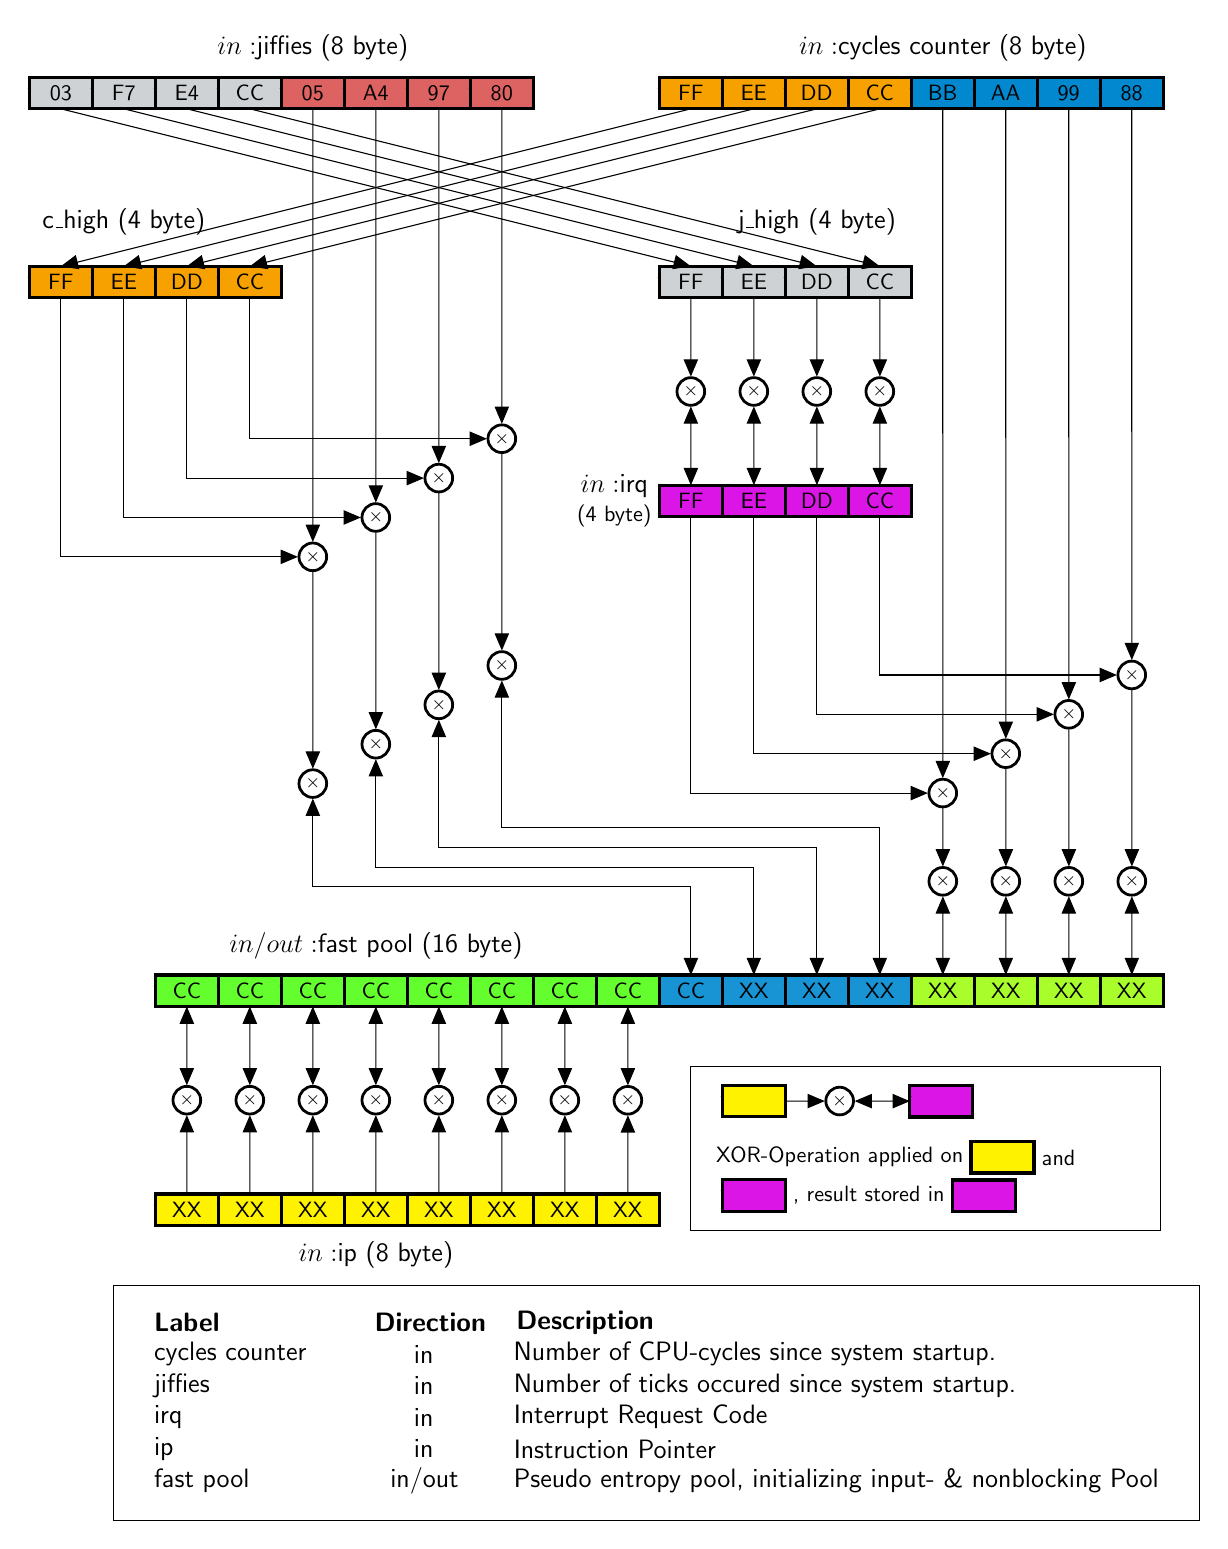
\begin{tikzpicture}[scale=0.8, every node/.style={scale=0.8},font=\sffamily,>=triangle 45]
	\tikzstyle{sum} = [draw, shape=circle, node distance=1.5cm, line width=1pt, minimum width=1.25em]	
	%\Huge
	\def\N{7}  % Number of Flip-Flops minus one
	\def\BW{1.8} % Byte Width

	% colors
	\definecolor{cjh}{HTML}{CFD2D4}
	\definecolor{cjl}{HTML}{DD6262}
	\definecolor{cch}{HTML}{F7A100}
	\definecolor{ccl}{HTML}{0288CF}
	\definecolor{cep32}{HTML}{64FE2E}
	\definecolor{cep1}{HTML}{1893D4}
	\definecolor{cep0}{HTML}{A9FD2A}
	\definecolor{cirq}{HTML}{DB15E5}
	\definecolor{cip}{HTML}{FFF200}

	% jiffies
	\node [shape=dff,fill=cjh] (jiff7) at ($ 1.0*(0,0) $) {03};
	\node [shape=dff,fill=cjh] (jiff6) at ($ 1.0*(1,0) $) {F7};
	\node [shape=dff,fill=cjh] (jiff5) at ($ 1.0*(2,0) $) {E4};
	\node [shape=dff,fill=cjh] (jiff4) at ($ 1.0*(3,0) $) {CC};			
	\node [shape=dff,fill=cjl] (jiff3) at ($ 1.0*(4,0) $) {05};
	\node [shape=dff,fill=cjl] (jiff2) at ($ 1.0*(5,0) $) {A4};
	\node [shape=dff,fill=cjl] (jiff1) at ($ 1.0*(6,0) $) {97};
	\node [shape=dff,fill=cjl] (jiff0) at ($ 1.0*(7,0) $) {80};	
	\node[above=1mm of jiff3] (ljiffies) {\large $in:$jiffies (8 byte)};		

	% jiffies low XOR c_high - XOR nodes
	\node [sum, below=4.0cm of jiff0, draw] (xjlch0) {};
	\node [sum, below=4.5cm of jiff1, draw] (xjlch1) {};	
	\node [sum, below=5.0cm of jiff2, draw] (xjlch2) {};
	\node [sum, below=5.5cm of jiff3, draw] (xjlch3) {};	
	\node [rotate=45] at (xjlch0) (plus) {{\footnotesize$+$}};
	\node [rotate=45] at (xjlch1) (plus) {{\footnotesize$+$}};	
	\node [rotate=45] at (xjlch2) (plus) {{\footnotesize$+$}};
	\node [rotate=45] at (xjlch3) (plus) {{\footnotesize$+$}};
		
	% cycles
	\node [shape=dff,fill=cch] (cycl7) at ($ 1.0*(10,0) $) {FF};
	\node [shape=dff,fill=cch] (cycl6) at ($ 1.0*(11,0) $) {EE};
	\node [shape=dff,fill=cch] (cycl5) at ($ 1.0*(12,0) $) {DD};
	\node [shape=dff,fill=cch] (cycl4) at ($ 1.0*(13,0) $) {CC};			
	\node [shape=dff,fill=ccl] (cycl3) at ($ 1.0*(14,0) $) {BB};
	\node [shape=dff,fill=ccl] (cycl2) at ($ 1.0*(15,0) $) {AA};
	\node [shape=dff,fill=ccl] (cycl1) at ($ 1.0*(16,0) $) {99};
	\node [shape=dff,fill=ccl] (cycl0) at ($ 1.0*(17,0) $) {88};
	\node[above=1mm of cycl3] (lcycles) {\large $in:$cycles counter (8 byte)};	

	%c_high
	\node [shape=dff,fill=cch, below=2cm of jiff7, draw] (chigh3) {FF};
	\node [shape=dff,fill=cch, below=2cm of jiff6, draw] (chigh2) {EE};
	\node [shape=dff,fill=cch, below=2cm of jiff5, draw] (chigh1) {DD};
	\node [shape=dff,fill=cch, below=2cm of jiff4, draw] (chigh0) {CC};
	\node[above=3mm of chigh2] (lchigh) {\large c\_high (4 byte)};			

	%j_high
	\node [shape=dff,fill=cjh, below=2cm of cycl7, draw] (jiffh3) {FF};
	\node [shape=dff,fill=cjh, below=2cm of cycl6, draw] (jiffh2) {EE};
	\node [shape=dff,fill=cjh, below=2cm of cycl5, draw] (jiffh1) {DD};
	\node [shape=dff,fill=cjh, below=2cm of cycl4, draw] (jiffh0) {CC};
	\node[above=3mm of jiffh1] (ljhigh) {\large j\_high (4 byte)};			

	% jiffies high XOR irq - XOR nodes
	\node [sum, below=1.0cm of jiffh3, draw] (xjhi3) {};	
	\node [rotate=45] at (xjhi3) (plus) {{\footnotesize$+$}};
	\node [sum, below=1.0cm of jiffh2, draw] (xjhi2) {};	
	\node [rotate=45] at (xjhi2) (plus) {{\footnotesize$+$}};
	\node [sum, below=1.0cm of jiffh1, draw] (xjhi1) {};	
	\node [rotate=45] at (xjhi1) (plus) {{\footnotesize$+$}};
	\node [sum, below=1.0cm of jiffh0, draw] (xjhi0) {};	
	\node [rotate=45] at (xjhi0) (plus) {{\footnotesize$+$}};
			
	%irq
	\node [shape=dff,fill=cirq, below=1cm of xjhi3, draw] (irq3) {FF};
	\node [shape=dff,fill=cirq, below=1cm of xjhi2, draw] (irq2) {EE};
	\node [shape=dff,fill=cirq, below=1cm of xjhi1, draw] (irq1) {DD};
	\node [shape=dff,fill=cirq, below=1cm of xjhi0, draw] (irq0) {CC};
	\node[left=0mm of irq3] (lirq) {\shortstack{\large $in:$irq\\(4 byte)}};	
	
	% cycles low XOR irq - XOR nodes
	\node [sum, below=8.5cm of cycl3, draw] (xcli3) {};
	\node [sum, below=8.0cm of cycl2, draw] (xcli2) {};	
	\node [sum, below=7.5cm of cycl1, draw] (xcli1) {};		
	\node [sum, below=7.0cm of cycl0, draw] (xcli0) {};			
	\node [rotate=45] at (xcli3) (plus) {{\footnotesize$+$}};
	\node [rotate=45] at (xcli2) (plus) {{\footnotesize$+$}};	
	\node [rotate=45] at (xcli1) (plus) {{\footnotesize$+$}};
	\node [rotate=45] at (xcli0) (plus) {{\footnotesize$+$}};	
	
	% entropy pool	
	\node [shape=dff,fill=cep32, below=11cm of jiff5, draw] (entp15) {CC};		
	\node [shape=dff,fill=cep32, below=11cm of jiff4, draw] (entp14) {CC};
	\node [shape=dff,fill=cep32, below=11cm of jiff3, draw] (entp13) {CC};
	\node [shape=dff,fill=cep32, below=11cm of jiff2, draw] (entp12) {CC};
	\node [shape=dff,fill=cep32, below=11cm of jiff1, draw] (entp11) {CC};
	\node [shape=dff,fill=cep32, below=11cm of jiff0, draw] (entp10) {CC};
	\node [shape=dff,fill=cep32, right=0cm of entp10, draw] (entp9) {CC};	
	\node [shape=dff,fill=cep32, right=0cm of entp9, draw] (entp8) {CC};
	\node [shape=dff,fill=cep1, right=0cm of entp8, draw] (entp7) {CC};
	\node [shape=dff,fill=cep1, below=11cm of cycl6, draw] (entp6) {XX};	
	\node [shape=dff,fill=cep1, below=11cm of cycl5, draw] (entp5) {XX};	
	\node [shape=dff,fill=cep1, below=11cm of cycl4, draw] (entp4) {XX};	
	\node [shape=dff,fill=cep0, below=11cm of cycl3, draw] (entp3) {XX};	
	\node [shape=dff,fill=cep0, below=11cm of cycl2, draw] (entp2) {XX};	
	\node [shape=dff,fill=cep0, below=11cm of cycl1, draw] (entp1) {XX};	
	\node [shape=dff,fill=cep0, below=11cm of cycl0, draw] (entp0) {XX};	
	\node[above=1mm of entp12] (lentp) {\large $in/out:$fast pool (16 byte)};	

	%% XOR entp
	% ch / jl 
	\node [sum, below=2.5cm of xjlch3, draw] (xentp7) {};	
	\node [rotate=45] at (xentp7) (plus) {{\footnotesize$+$}};
	\node [sum, below=2.5cm of xjlch2, draw] (xentp6) {};	
	\node [rotate=45] at (xentp6) (plus) {{\footnotesize$+$}};
	\node [sum, below=2.5cm of xjlch1, draw] (xentp5) {};	
	\node [rotate=45] at (xentp5) (plus) {{\footnotesize$+$}};
	\node [sum, below=2.5cm of xjlch0, draw] (xentp4) {};	
	\node [rotate=45] at (xentp4) (plus) {{\footnotesize$+$}};									
	% irq/cycl 
	\node [sum, above=1.0cm of entp3, draw] (xentp3) {};	
	\node [rotate=45] at (xentp3) (plus) {{\footnotesize$+$}};
	\node [sum, above=1.0cm of entp2, draw] (xentp2) {};	
	\node [rotate=45] at (xentp2) (plus) {{\footnotesize$+$}};
	\node [sum, above=1.0cm of entp1, draw] (xentp1) {};	
	\node [rotate=45] at (xentp1) (plus) {{\footnotesize$+$}};
	\node [sum, above=1.0cm of entp0, draw] (xentp0) {};	
	\node [rotate=45] at (xentp0) (plus) {{\footnotesize$+$}};		
	% ip
	\node [sum, below=1.0cm of entp15, draw] (xentp15) {};	
	\node [rotate=45] at (xentp15) (plus) {{\footnotesize$+$}};
	\node [sum, below=1.0cm of entp14, draw] (xentp14) {};	
	\node [rotate=45] at (xentp14) (plus) {{\footnotesize$+$}};
	\node [sum, below=1.0cm of entp13, draw] (xentp13) {};	
	\node [rotate=45] at (xentp13) (plus) {{\footnotesize$+$}};
	\node [sum, below=1.0cm of entp12, draw] (xentp12) {};	
	\node [rotate=45] at (xentp12) (plus) {{\footnotesize$+$}};		
	\node [sum, below=1.0cm of entp11, draw] (xentp11) {};	
	\node [rotate=45] at (xentp11) (plus) {{\footnotesize$+$}};
	\node [sum, below=1.0cm of entp10, draw] (xentp10) {};	
	\node [rotate=45] at (xentp10) (plus) {{\footnotesize$+$}};
	\node [sum, below=1.0cm of entp9, draw] (xentp9) {};	
	\node [rotate=45] at (xentp9) (plus) {{\footnotesize$+$}};
	\node [sum, below=1.0cm of entp8, draw] (xentp8) {};	
	\node [rotate=45] at (xentp8) (plus) {{\footnotesize$+$}};	

	\node [shape=dff,fill=cip, below=1cm of xentp15, draw] (ip7) {XX};	
	\node [shape=dff,fill=cip, below=1cm of xentp14, draw] (ip6) {XX};
	\node [shape=dff,fill=cip, below=1cm of xentp13, draw] (ip5) {XX};
	\node [shape=dff,fill=cip, below=1cm of xentp12, draw] (ip4) {XX};
	\node [shape=dff,fill=cip, below=1cm of xentp11, draw] (ip3) {XX};
	\node [shape=dff,fill=cip, below=1cm of xentp10, draw] (ip2) {XX};
	\node [shape=dff,fill=cip, below=1cm of xentp9, draw] (ip1) {XX};
	\node [shape=dff,fill=cip, below=1cm of xentp8, draw] (ip0) {XX};
	\node[below=1mm of ip4] (lip) {\large $in:$ip (8 byte)};	

	%%%%%% LINES >>
	
	% jiffies  -> c_low - lines
	\draw [->] (jiff3.south) -- (xjlch3.north);
	\draw [->] (jiff2.south) -- (xjlch2.north);	
	\draw [->] (jiff1.south) -- (xjlch1.north);		
	\draw [->] (jiff0.south) -- (xjlch0.north);		

	% c_high -> xjlch
	\draw [->] (chigh3.south)|- (xjlch3.west);
	\draw [->] (chigh2.south)|- (xjlch2.west);
	\draw [->] (chigh1.south)|- (xjlch1.west);
	\draw [->] (chigh0.south)|- (xjlch0.west);			

	% jiffies high -> j_high
	\draw [->] (jiff7.south) -- (jiffh3.north);
	\draw [->] (jiff6.south) -- (jiffh2.north);	
	\draw [->] (jiff5.south) -- (jiffh1.north);		
	\draw [->] (jiff4.south) -- (jiffh0.north);		

	% cycles_high -> c_high
	\draw [->] (cycl7.south) -- (chigh3.north);
	\draw [->] (cycl6.south) -- (chigh2.north);	
	\draw [->] (cycl5.south) -- (chigh1.north);		
	\draw [->] (cycl4.south) -- (chigh0.north);		
	
	% cycles_low -> c_high
	\draw [->] (cycl3.south) -- (xcli3.north);
	\draw [->] (cycl2.south) -- (xcli2.north);	
	\draw [->] (cycl1.south) -- (xcli1.north);		
	\draw [->] (cycl0.south) -- (xcli0.north);	

	% jiffies high -> j_high
	\draw [->] (jiffh3.south) -- (xjhi3.north);
	\draw [->] (jiffh2.south) -- (xjhi2.north);	
	\draw [->] (jiffh1.south) -- (xjhi1.north);		
	\draw [->] (jiffh0.south) -- (xjhi0.north);
		
	% xjhi -> irq
	\draw [<->] (xjhi3.south) -- (irq3.north);
	\draw [<->] (xjhi2.south) -- (irq2.north);	
	\draw [<->] (xjhi1.south) -- (irq1.north);		
	\draw [<->] (xjhi0.south) -- (irq0.north);
	
	% xjlch -> xentp
	\draw [->] (xjlch3.south) -- (xentp7.north);
	\draw [->] (xjlch2.south) -- (xentp6.north);	
	\draw [->] (xjlch1.south) -- (xentp5.north);		
	\draw [->] (xjlch0.south) -- (xentp4.north);

	% irq -> xcli
	\draw [->] (irq3.south) |- (xcli3.west);
	\draw [->] (irq2.south) |- (xcli2.west);	
	\draw [->] (irq1.south) |- (xcli1.west);		
	\draw [->] (irq0.south) |- (xcli0.west);

	% xentp -> entp
	\draw [<->] (xentp7.south) |- ($(entp7.north)!1/2!(entp7.north |- xentp7.south)$) coordinate (C1) -| (entp7.north);			
	\draw [<->] (xentp6.south) |- ($(entp6.north)!1/2!(entp6.north |- xentp6.south)$) coordinate (C2) -| (entp6.north);		
	\draw [<->] (xentp5.south) |- ($(entp5.north)!1/2!(entp5.north |- xentp5.south)$) coordinate (C3) -| (entp5.north);				
	\draw [<->] (xentp4.south) |- ($(entp4.north)!1/2!(entp4.north |- xentp4.south)$) coordinate (C4) -| (entp4.north);	
	
	% xcli -> xentp
	\draw [->] (xcli3.south) -- (xentp3.north);
	\draw [->] (xcli2.south) -- (xentp2.north);	
	\draw [->] (xcli1.south) -- (xentp1.north);		
	\draw [->] (xcli0.south) -- (xentp0.north);	

	% xcli -> xentp
	\draw [<->] (xentp3.south) -- (entp3.north);
	\draw [<->] (xentp2.south) -- (entp2.north);	
	\draw [<->] (xentp1.south) -- (entp1.north);		
	\draw [<->] (xentp0.south) -- (entp0.north);
	
	% xentp -> entp
	\draw [<->] (xentp15.north) -- (entp15.south);
	\draw [<->] (xentp14.north) -- (entp14.south);
	\draw [<->] (xentp13.north) -- (entp13.south);
	\draw [<->] (xentp12.north) -- (entp12.south);
	\draw [<->] (xentp11.north) -- (entp11.south);
	\draw [<->] (xentp10.north) -- (entp10.south);
	\draw [<->] (xentp9.north) -- (entp9.south);
	\draw [<->] (xentp8.north) -- (entp8.south);
	
	% ip -> xentp
	\draw [->] (ip7.north) -- (xentp15.south);
	\draw [->] (ip6.north) -- (xentp14.south);
	\draw [->] (ip5.north) -- (xentp13.south);
	\draw [->] (ip4.north) -- (xentp12.south);
	\draw [->] (ip3.north) -- (xentp11.south);
	\draw [->] (ip2.north) -- (xentp10.south);
	\draw [->] (ip1.north) -- (xentp9.south);
	\draw [->] (ip0.north) -- (xentp8.south);
	
	%%%%%% Legende 
\begin{scope}
	\node [shape=dff,fill=cip, below=10mm of entp6, draw] (f8) {};
	\node [sum, right=5mm of f8, draw] (xf8) {};	
	\node [rotate=45] at (xf8) (plus) {{\footnotesize$+$}};	
	\node [shape=dff,fill=cirq, right=7mm of xf8, draw] (c3) {};
	\draw [->] (f8.east) -- (xf8.west);
	\draw [<->] (xf8.east) -- (c3.west);
	\node[black, below=3mm of xf8, align=left] (lf81) {XOR-Operation applied on};	
	\node [shape=dff,fill=cip, right=0mm of lf81, draw] (rf8) {};
	\node[black, right=0mm of rf8, align=left] (lf82) {and};	
	
	\node [shape=dff,fill=cirq, below=22mm of entp6, draw] (yf8) {};
	\node[black, right=0mm of yf8, align=left] (lf83) {, result stored in};
	\node [shape=dff,fill=cirq, right=0mm of lf83, draw] (zf8) {};	
	\draw[black] ([xshift=-5mm, yshift=3mm ]f8.north west) rectangle ([xshift=23mm, yshift=-3mm]zf8.south east);	
\end{scope}	

\begin{scope}
\large
%\node [draw, align=center] {Text\\und Text};
\node[black, below=10mm of ip7, align=left] (lghdlbl) {\textbf{Label}};	
\node[black, right=28mm of lghdlbl.west, anchor=west, align=left] (lghddirr) {\textbf{Direction}};
\node[black, right=18mm of  lghddirr.west, anchor=west, align=left] (lghddesc) {\textbf{Description}};

%\node[black, below=10mm of ip4, align=left] (lgjif) {\textbf{cycles counter}};	
\node[black, below=4mm of lghdlbl.west, anchor=west, align=left] (lgcc) {cycles counter};	
\node[black, below=4mm of lgcc.west, anchor=west] (lgjif) {jiffies};	
\node[black, below=4mm of lgjif.west, anchor=west] (lgirq) {irq};	
\node[black, below=4mm of lgirq.west, anchor=west] (lgip) {ip};
\node[black, below=4mm of lgip.west, anchor=west] (lgentp) {fast pool};

\node[black, right=33mm of lgcc.west, align=left] (lgdircc) {in};	
\node[black, right=33mm of lgjif.west, align=left] (lgdirjif) {in};	
\node[black, right=33mm of lgirq.west, align=left] (lgdirirq) {in};
\node[black, right=33mm of lgip.west, align=left] (lgdirip) {in};
\node[black, right=30mm of lgentp.west, align=center] (lgdientp) {in/out};


\node[black, right=24mm of lgcc, align=left] (lgcctxt) {Number of CPU-cycles since system startup.};	
\node[black, below=4mm of lgcctxt.west, anchor=west] (lgjiftxt) {Number of ticks occured since system startup.};	
\node[black, below=4mm of lgjiftxt.west, anchor=west] (lgirqtxt) {Interrupt Request Code};
\node[black, below=4mm of lgirqtxt.west, anchor=west] (lgiptxt) {Instruction Pointer};
\node[black, below=4mm of lgiptxt.west, anchor=west] (lgentptxt) {Pseudo entropy pool, initializing input- \& nonblocking Pool};

\draw[black] ([xshift=-5mm, yshift=3mm ]lghdlbl.north west) rectangle ([xshift=5mm, yshift=-3mm]lgentptxt.south east);
	
\end{scope}
\end{tikzpicture}
\caption{Processing of input parameters by func. 'add\_interrupt\_randomness' before applying fast\_mix / mix\_pool\_bytes operations (valid for 64-bit Kernel only)} \label{fig:add-int-rnd-chart}
\end{figure}


%\begin{mdframed}
%\begin{tabularx}{\columnwidth}{XXl}
%\begin{tabularx}{\textwidth}{ll}
%%	\caption{Description of input parameters proccessed by func. 'add\_interrupt\_randomness'}
%%	\label{tab:add-int-rnd-desc}\\
%	\textbf{jiffies}&Igel\\
%	\textbf{cycles counter}&Dienstag\\
%	\textbf{irq}&\\
%	\textbf{ip}&\textit{Instruction Pointer}
%	\caption{Description of input parameters proccessed by func. 'add\_interrupt\_randomness'}
%\end{tabularx}
%\centering
%\begin{table}[H]
%	\begin{tabular}{ll}
%	\textbf{Jiffies}&Nr. of ticks occured since system startup.\\
%	\textbf{Cycles Counter}&Nr. of CPU-cycles since system startup.\\
%	\textbf{irq}&Interrupt Request \\
%	\textbf{ip}&\textit{Instruction Pointer}
%	\end{tabular}
%	\caption{Description of input parameters proccessed by func. 'add\_interrupt\_randomness'}	
%\end{table}

% jiffies . Incremented for each timer interrupt.
% . also known as \textit{Time Stamp Counter}.

%	\cite{kernlrandmc}
		
%\end{mdframed}


%\begin{tabularx}{\columnwidth}{XXl}
%	jiffies&Schnecke&Igel\\
%	cycles counter&Hier ist ein langes Wort Hier ist ein langes Wort Hier ist ein langes Wort Hier ist ein langes Wort &Dienstag\\
%	irq&&\\
%	ip&&
%\end{tabularx}
%
%
%
%\begin{mdframed}
%\begin{description}
%	\item [jiffies] sadfasdfsadf
%	\item [cycles counter] asdfasdfasdf
%	\item [irq] asdfasdfasdf	
%	\item [ip] 
%\end{description}
%\cite{kernlrandmc}	
%\end{mdframed}




\section{Conclusion}
The final section of the chapter gives an overview of the important results
of this chapter. This implies that the introductory chapter and the
concluding chapter don't need a conclusion.

\lipsum[66]

%%% Local Variables: 
%%% mode: latex
%%% TeX-master: "thesis"
%%% End: 

\chapter{Random Number Generation in Linux x64 Kernel 4.4}
\label{cha:3}

\section{General}\label{sec:lrng-general}

Random numbers are required by a variety of security related applications. An obvious purpose is encryption or signing of data, like f.e. disk encryption, Transport Socket Layer (TLS) or digital signatures of emails. In this case random numbers are used to generate cryptographically secure keys. Concepts like Stack Canaries (aka. Stack Guards) or Address Space Layout Randomization (ASLR) rely purely on the nondeterministic character of random numbers, applying them to make certain types of attacks on vulnerable applications much more difficult. Overall, the effectiveness of such applications depends significantly on the quality i.e. unpredictably of random numbers, provided by an operating system. \\
In the following, a comprehensive introduction to the Linux Random Number Generator (LRNG) with focus on analyzed concepts and components of this thesis will be given. It refers to Linux kernel v.4.4, which is currently used in several major Long Term Support distributions like Ubuntu Server 16.04 LTS. If facts are valid for Intel x86/x64 platforms only, those will be noted as such.
As the analysis of random numbers i.e. their quality in terms of entropy will be analyzed compliant to an approach (\cite{turan2018nist}) recommended by the National Institute of Standards and Technology the corresponding terminology will be used.\\
In general, many modern CPU-architectures implement an on-chip True Random Number Generators. Starting with 'IvyBridge' architecture, Intel provides two instructions accessing directly those entropy sources. The \textsf{RDRAND} instruction returns random numbers that are supplied by a cryptographically secure, deterministic random bit generator which is designed to meet the NIST SP 800-90A standard. If an application or operating system design insists on applying in it's own Pseudo Random Number Generator (PRNG) it may apply the \textsf{RDSEED} instruction which is compliant to NIST SP 800-90B \& C standard \cite{guide2017intel} for initializing i.e. seeding its state.
Availability of these TRNGs does not automatically imply their application. If a kernel is started 
with paramter \textsf{nordrand} (on x86/x64 architectures), the \textsf{RDRAND} instruction will have no effect. Further, if an operating system is run as a virtual machine, those instructions can by trapped by the hypervisor instead of being passed to the CPU \cite{mueller@bsi2}. Thus, the analysis in this thesis does not take on-chip entropy pools into account, but refers to the pure Linux Pseudo Random Number Generator.

\section{Linux Pseudo Random Number Generator Architecture Overview}\label{sec:lrng-arch}
The Linux Pseudo Random Number Generator's (PRNG) responsibility is for providing random numbers to requesting consumers. To ensure a certain quality of randomness the implementation's activity is  divided into four major tasks:   

%\begin{figure}
\begin{itemize}
	\item Capturing and processing of input data which is finally stored in entropy pools or buffers
	\item Assessing and health checking the level of entropy in each pool in unit 'bits of entropy'
	\item Diverting incoming entropy to specific pools, depending on a pool's state
	\item Releasing random numbers to a consumer 
\end{itemize}
%	\caption{Major tasks of the Linux PRNG}
%\end{figure}
Depending on the type of consumer, there is a fundamental difference in the way random numbers can be requested. Applications or services running in user mode access those via different interfaces than logic running with kernel privileges does. Also, the source of entropy varies vastly, depending on the consumer type. The security components analyzed in this thesis are involved in the generation of new processes. This task is accomplished by code running on kernel level, hence the initialization and management of entropy sources for this consumer type are in focus of this introduction, but partly overlap with those dedicated to user mode consumers.
\\~\\
To generate random numbers, the Linux PRNG needs to fall back on events delivered by hardware. 
Capturing and processing of several types of hardware events starts immediately after the kernel has been loaded into memory and is given execution by the boot loader. With the occurrence of each type of hardware event, pre-processing routines (more or less sophisticated transformations) are applied on the delivered input parameters. Those may be as simple as a single XOR- or ADD-operation to more complex but lean transformations, partly reinvolving previously calculated results. The outcome of these operations is finally assigned to entropy pools. An entropy pool is a data structure located in kernel memory. Beside storing the generated random numbers, it is also aware of its entropy state. Depending on its purpose, an entropy pool delivers data to a consumer interface, or is meant to enrich other pools. In total, in the Linux kernel exist three full-featured entropy pools which will be explained in the following. Some hardware events are processed by a so called fast\_pool, which must be seen as a pre-processing stage instead of a full-featured entropy pool \cite{mueller@bsi2}. Additionally, part of the initialization process is the set up of a 16 byte vector, which is assigned once during system startup. This vector is involved as a seed for conditioning i.e. more sophisticated transformations like MD5 or SHA2, applied on kernel level consumers' requests of random numbers. Hence the development of this vector is of particular interest for this thesis. Figure \ref{fig:linux-prng-arch} illustrates all major components involved in the generation and management of random numbers via the Linux PRNG. The following sections will explain their dedication and interaction more briefly.

\begin{figure}[H]
	\centering
	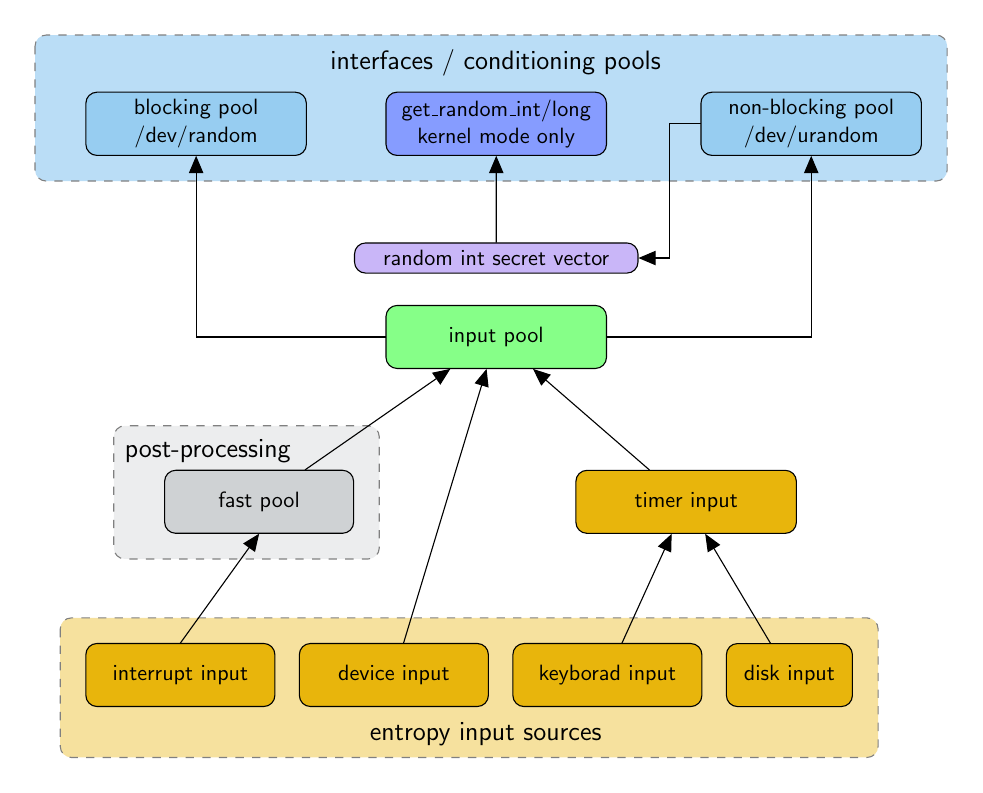
\begin{tikzpicture}[scale=0.8, every node/.style={scale=0.8},font=\sffamily,>=triangle 45]
\tikzstyle{sum} = [draw, shape=circle, node distance=1.5cm, line width=1pt, minimum width=1.25em]	
%\Huge
\def\N{7}  % Number of Flip-Flops minus one
\def\BW{1.8} % Byte Width

% colors
\definecolor{rc-input}{HTML}{E8B50C}
\definecolor{gr-input}{HTML}{E8B50C}
\definecolor{rc-input-pool}{HTML}{0DFF11}
\definecolor{rc-user-pool}{HTML}{52ABE8}
\definecolor{rc-kernel-pool}{HTML}{0D38FF}
\definecolor{rc-fast-pool-col}{HTML}{CFD2D4}
\definecolor{rc-rnd-int-sec-vect-col}{HTML}{4B0CE8}
%4B0CE8

%4B0CE8
%B8FFF7

\definecolor{cjh}{HTML}{CFD2D4}
\definecolor{cjl}{HTML}{DD6262}
\definecolor{cch}{HTML}{F7A100}
\definecolor{ccl}{HTML}{0288CF}
\definecolor{cep32}{HTML}{64FE2E}
\definecolor{cep1}{HTML}{1893D4}
\definecolor{cep0}{HTML}{A9FD2A}
\definecolor{cirq}{HTML}{DB15E5}
\definecolor{cip}{HTML}{FFF200}

% blocing pool
%\node [shape=dff,fill=cjh, width=30mm] (jiff7) at ($ 1.0*(0,0) $) {blocking pool};
% rect rc-blocking-pool
\node (rc-blocking-pool) [rectangle, rounded corners, fill=rc-user-pool!60, draw, minimum width=35mm, minimum height=10mm, anchor= south west] at (0,0) {\shortstack{blocking pool\\/dev/random}};
% rect get_random_int/long
\node (rc-getrandomintlong) [rectangle, rounded corners, right=10mm of rc-blocking-pool, fill=rc-kernel-pool!50, draw, minimum width=35mm, minimum height=10mm, anchor= west] {\shortstack{get\_random\_int/long\\kernel mode only}};		
% rect rc-nonblocking-pool
\node (rc-nonblocking-pool) [rectangle, rounded corners, right=50mm of rc-blocking-pool, fill=rc-user-pool!60, draw, minimum width=35mm, minimum height=10mm, anchor= west] {\shortstack{non-blocking pool\\/dev/urandom}};	
% rect rc-input-pool	
\node (rc-input-pool) [rectangle, rounded corners, below right=23mm and 10mm of rc-blocking-pool, fill=rc-input-pool!50, draw, minimum width=35mm, minimum height=10mm, anchor= west] {input pool};
% rc-input-pool -> rect rc-blocking-pool
\draw [->] (rc-input-pool.west) -| (rc-blocking-pool);	
% rc-input-pool -> rect rc-nonblocking-pool
\draw [->] (rc-input-pool.east) -| (rc-nonblocking-pool);	
% rect rc-rnd-int-sec	
\node (rc-rnd-int-sec) [rectangle, rounded corners, above=4mm of rc-input-pool.north, fill=rc-rnd-int-sec-vect-col!30, draw, minimum width=45mm, minimum height=3mm] {random int secret vector};
% rc-nonblocking-pool -> rc-rnd-int-sec
\draw [<-] (rc-rnd-int-sec.east) -| ($(rc-nonblocking-pool.west)!1/2!(rc-nonblocking-pool.west -| rc-rnd-int-sec.east)$) coordinate (C4) -| (rc-nonblocking-pool.west);
% rc-rnd-int-sec -> rect get_random_int/long
\draw [->] (rc-rnd-int-sec.north) -- (rc-getrandomintlong.south);
\node[above right=5mm and -8mm of rc-getrandomintlong.west] (lentp) {\large interfaces / conditioning pools };
\begin{pgfonlayer}{background}
% background - pre-processing
\path (rc-blocking-pool.west |- rc-blocking-pool.north)+(-0.8,0.9) node (a) {};
\path (rc-nonblocking-pool.east |- rc-nonblocking-pool.south)+(0.4,-0.4) node (b) {};
\path [fill=rc-user-pool!40,rounded corners, draw=black!50, dashed] (a) rectangle (b); 
\end{pgfonlayer}
		

%	\draw [->] (rc-nonblocking-pool.west) -| (rc-rnd-int-sec.north);

% rect rc-interrupt-inp
\node (rc-interrupt-inp) [rectangle, rounded corners, below=70mm of rc-blocking-pool.west, fill=rc-input, draw, minimum 
width=30mm, minimum height=10mm, anchor= west] {\shortstack{interrupt input}};
% rect rc-device-inp	
\node (rc-device-inp) [rectangle, rounded corners, right=3mm of rc-interrupt-inp.east, fill=rc-input, draw, minimum width=30mm, minimum height=10mm, anchor= west] {\shortstack{device input}};
% rect rc-key-inp	
\node (rc-key-inp) [rectangle, rounded corners, right=3mm of rc-device-inp.east, fill=rc-input, draw, minimum width=30mm, minimum height=10mm, anchor= west] {\shortstack{keyborad input}};
% rect rc-disk-inp	
\node (rc-disk-inp) [rectangle, rounded corners, right=3mm of rc-key-inp.east, fill=rc-input, draw, minimum width=20mm, minimum height=10mm, anchor= west] {\shortstack{disk input}};

% rect rc-fast-pool	
\node (rc-fast-pool) [rectangle, rounded corners, above right=22mm and 10mm of rc-interrupt-inp.west, fill=rc-fast-pool-col, draw, minimum width=30mm, minimum height=10mm, anchor= west] {\shortstack{fast pool}};
% rc-interrupt-inp -> rc-fast-pool
\draw [->] (rc-interrupt-inp.north) -- (rc-fast-pool.south);
% rc-fast-pool -> rc-input-pool
\draw [->] (rc-fast-pool) -- (rc-input-pool);
% rc-device-inp -> rc-input-pool
\draw [->] (rc-device-inp) -- (rc-input-pool);
\node[above right=4mm and -6mm of rc-fast-pool.west] (lentp) {\large post-processing};
\begin{pgfonlayer}{background}
% background - pre-processing
\path (rc-fast-pool.west |- rc-fast-pool.north)+(-0.8,0.7) node (a) {};
\path (rc-fast-pool.east |- rc-fast-pool.south)+(0.4,-0.4) node (b) {};
\path [fill=rc-fast-pool-col!40,rounded corners, draw=black!50, dashed] (a) rectangle (b); 
\end{pgfonlayer}


rc-fast-pool-col

% rect rc-timer-inp	
\node (rc-timer-inp) [rectangle, rounded corners, above right=22mm and 8mm of rc-key-inp.west, fill=rc-input, draw, minimum width=35mm, minimum height=10mm, anchor= west] {timer input};	
% rc-key-inp -> rc-timer-inp
\draw [->] (rc-key-inp) -- (rc-timer-inp);
% rc-disk-inp -> rc-timer-inp
\draw [->] (rc-disk-inp) -- (rc-timer-inp);
% rc-timer-inp -> rc-input-pool
\draw [->] (rc-timer-inp) -- (rc-input-pool);

\node[below right=5mm and 8mm of rc-device-inp.west] (lentp) {\large entropy input sources};
\begin{pgfonlayer}{background}
% background - entropy input sources
\path (rc-interrupt-inp.west |- rc-interrupt-inp.north)+(-0.4,0.4) node (a) {};
\path (rc-disk-inp.east |- rc-disk-inp.south)+(0.4,-0.8) node (b) {};
\path [fill=gr-input!40,rounded corners, draw=black!50, dashed] (a) rectangle (b); 
\end{pgfonlayer}


\end{tikzpicture}		

	\caption{Input sources and entropy pools, -vectors, interfaces of the Linux PRNG} 
	\label{fig:linux-prng-arch}
\end{figure}

\section{Input sources of the Linux PRNG}
In best case, the generation of random numbers is conducted by dedicated devices in terms of True Random Number Generators. The Linux RNG implementation allows to involve TRNGs in two ways: 
\begin{itemize}
	\item \textit{Instruction Delegation:} Requests from consumers are directly translated into instructions using architecture dependent on-chip features as described in \ref{sec:lrng-general}.
	This approach bypasses the entire logic of the Linux PRNG and relies completely on the TRNG.
	\item \textit{TRNG/PRNG Hybrid Mode:} Random numbers are managed via the regular PRNG logic. Instead of transformed hardware events, the entropy pools are filled with data, provided by a TRNG device via a special driver interface.
\end{itemize}
For this thesis, both of these options are out of scope. Instead, the process of generating random numbers based on common hardware events is analyzed. As an outcome, it turned out that just two types of hardware events were able to provide input data, while the reaming did not contribute anything at all, since the operating system was run as a virtual machine. Despite this, also those should be mentioned for the sake of completeness.

\subsection{Timing Variance}
For each hardware event type a data structure \textsf{timer\_rand\_state} is maintained tracking the occurrence of events. Depending on the event type, this information will used to enrich the 
input pool via passing it's value to \textsf{add\_timer\_randomness} and/or to discard the event parameter if a minimum interval has not pass yet. 

\subsection{Input Randomness}\label{sec:inp-rnd}
Input events comprise any kind of parameters delivered by user input devices like a keyboard or a mouse. A keyboard the usually delivers the keycode, a mouse the coordinate of the cursor position. However the devices need to be connected locally \cite{mueller@bsi2}. Since this does not apply a an operating system run as a virtual machine, \textsf{add\_input\_randomness} is never called and further also no timer input is delivered to \textsf{add\_timer\_randomness} by this type of event.

\subsection{Disk Randomness}\label{sec:disk-rnd}
Per disk i.e. block device the amount of seek time of a block layer request  \textsf{add\_disk\_randomness} will contribute to the input pool via a call of \textsf{add\_timer\_randomness}. However, if a virtual machine is hosted on a solid state drives timing variance of events is to low and constant. Hence also this event type does not deliver any noise for this setup.

\subsection{Device Randomness}\label{sec:dev-rnd}
Function \textsf{add\_device\_randomness} is called just one, in a very early phase, when the kernel starts to initialize device drivers. In the applied virtual environment this event type's parameters where limited on BIOS/UEFI related information like manufacture name, vendor-id and the serial number. This information commonly is static. While at least some parameters may be individual on a hardware installation, the Xen-Hypervisor allows to use an identical BIOS/UEFI image for arbitrary virtual machines.   

\subsection{Interrupt Randomness}\label{sec:int-rnd}
Via the concept of interrupts, system components are enabled to request an interrupt of the system's current activity, to deliver or demand information. When an interrupt request (IRQ) is signaled, the system will halt at defined state, exchange data with requesting unit and finally or immediately proceed execution. The intention of a request is communicated via an IRQ-code. These codes are well known to the operating system, as predefined by convention and set by the BIOS. IRQ 0 f.e., signals a periodic occurring timer event. As illustrated in \ref{fig:linux-prng-arch}, detouring the fast pool, interrupt input initializes the input pool. As mentioned in \ref{sec:inp-rnd} and \ref{sec:disk-rnd}, disk- and input events don't contribute any noise at all, while entropy provided by \textsf{add\_device\_randomness} is assumed to be poor. In other words, the development of the input entropy pools depends significantly on the parameters provided by \textsf{add\_interrupt\_randomness} and is hence of particular interest, since this pool is finally responsible to initialize the \textsf{random\_int\_secret} vector, which is applied as seed for each request triggered by a kernel process. TODOC
%if ((fast_pool->count < 64) && !time_after(now, fast_pool->last + HZ))
% erwaehnen das add_interrupt_randomness abbricht wenn fast_pool->last + HZ

\section{Entropy Pools, Pre-Processing and Vectors}
An entropy pool is a complex data structure dedicated to store generated random values as well as its own state regarding the currently achieved entropy level. In total, in Linux Kernel 4.4 are existing three pools based on data structure \textsf{entropy\_store}, named blocking-pool, non-blocking-pool and input-pool (see \ref{fig:linux-prng-arch}) \cite{kernlrandmc}. The blocking- and non-blocking-pool are so called output pools, directly accessibly via applications or services running in \gls{usrmd}. By contrast, code running in \gls{knlmd} uses kernel internal functions \textsf{get\_random\_int} i.e. \textsf{get\_random\_long} to retrieve random values. Those consumer interfaces have a conditioning behavior in common, hence also called conditioning pool. When random numbers are requested 


\cite{damasevicius2012energy}

Beside, a pre-proccessing fast-post 


\subsection{Input Pool}\label{sub:input-pool}
512 byte \cite{kernlrandmc}
no interface 
sophisticated \gls{iotg}



\subsection{Fast Pools}
As mentioned in \ref{sec:lrng-arch}, fast pools are no full-featured entropy pools, but have the purpose of a pre-processing stage, dedicated to initialize the input pool. As illustrated in \ref{fig:linux-prng-arch}, fast pools are feed by noise delivered by interrupt event input. They are declared by a simple data structure, which is able to store 16 byte of gained random values beside few state information, as illustrated in \ref{fig:fast-pool}.\\
This data structure is instantiated and addressed per CPU, available to the operating system.
%TODO: Hier noch ein Verweis rein, das diese relativ fix sind (gelesen in mark..)??
 
 \begin{lstlisting}[caption=Declaration of the fast\_pool structure in Linux kernel 4.4 \cite{kernlrandmc}, captionpos=b,
 xrightmargin=.3\textwidth,
 xleftmargin=.3\textwidth,
 label=lst:fastspool]
 struct fast_pool {
    __u32 pool[4];
    unsigned long last;
    unsigned short reg_idx;
    unsigned char count;
 };
 \end{lstlisting}
 
 For this thesis, the number of available CPUs per virtual machine has been configured to one, hence the terminology will refer to a single instance in the following. By concept, in Linux Kernel 4.4, interrupt randomness is the sole source of random noise available to rise up the fast pool, which is a contributor to the input entropy pool. As observations of the experimental setup for this thesis concluded that beside interrupt events any contribution has occurred by input- or disk events. In other words, the development of the fast pool, depends completely on the input and pre-processing conducted by \textsf{add\_interrupt\_randomness} and hence will be will be described more briefly.\\
 For each call of function \textsf{add\_interrupt\_randomness}, several parameters are processed to transform the 16 byte vector of the fast pool (labeled 'pool' in \ref{fig:fast-pool}). Thereby just one of two parameters directly passed by the caller. Surprisingly parameter \textsf{irq\_code}, is processed, while the second, \textsf{irq\_flags} is used at all (see \ref{lst:add-interrupt-randomnes-c}), for unknown reasons. Beside this input, three more runtime values are applied on pre-proccessing procedures within the function. Some of them are also applied for Component processing by XXX TODO and will be explained more detailed.
 
 \begin{itemize}
 	\item \textbf{Cycles Counter [8 byte]} The cycles counter (see 'cycles' in  \ref{lst:add-interrupt-randomnes-c}) is a high-resolution counter of 8 byte length (on x64 plattforms), used to receive CPU timing information. It is also referred as Time Stamp Counter and is invokable via the \textsf{RDTSC} instruction \cite{guide2017intel}. Cycles Counter is managed by the CPU which monotonically increments the time-stamp counter model-specific register (MSR) every clock cycle and resets it to 0 whenever	the processor is reset. As mentioned in TODO the results retrieved by the calling \textsf{RDTSC} instruction may not be directly passed to the CPU but deliver emulation based results, depending on the Xen configuration setting \textsf{tsc\_mode} \cite{xentscmode} for a particular virtual machine. For the given Virtual Environment Setup of this thesis, per default, the cycles counter value has been provided by the underlying CPU to both virtual machines.
 	
	\item \textbf{Instruction Pointer [8 byte]} On x64 platforms, the instruction pointer (see 'ip' in \ref{lst:add-interrupt-randomnes-c}) holds the 64-bit offset of the next
	instruction to be executed, which is hold in CPU-register RIP. This architecture also support a technique called RIP-relative addressing. Using this technique, the effective address is determined by adding a displacement to the RIP of the next instruction \cite{guide2017intel}.
	
	\item \textbf{Jiffies [8 byte]} Jiffies (see 'now' in \ref{lst:add-interrupt-randomnes-c}) represent a kernel-internal value which is incremented at each timer interrupt. This counter may be seen as some kind of software clock maintained by the kernel which measures time in jiffies \cite{timeandtimers}. The accuracy of jiffies is determined by the value of the kernel compile-time constant \textsf{HZ} TODO Ref. On system startup, jiffies is initialized to an initial value.
	
 \end{itemize}
 
 
 \subsection{get\_random\_int/\_long}
 
 MD5-transform
 
 %TODO (nachhaken-soll das rein?)
 
%  in 
% \ref{sub:input-pool}
 
 %enrichment
 
% Pre-processing
%fast_pool
% \textsf{add\_interrupt\_randomness}
%struct fast_pool {
%	__u32		pool[4];
%	unsigned long	last;
%	unsigned short	reg_idx;
%	unsigned char	count;
%};

%
%{sec:int-rnd}
%one per CPU
%XOR 
%solely


%\begin{lstlisting}[float, caption={declares of the fast_pool structure},captionpos=b, xleftmargin=.4\textwidth]
%struct fast_pool {
%__u32		pool[4];
%unsigned long	last;
%unsigned short	reg_idx;
%unsigned char	count;
%};
%\end{lstlisting}




%\textsf{add\_interrupt\_randomness}



% In total there are X types 

% Those will be explained in XXX and YYY.  



%generates random numbers based on occurring hardware events. Those events 


\begin{comment}
Jegliche Nutzung der RDRAND-Instruktion kann verhindert werden, wenn der Kern mit der
Kommandozeilenoption ?nordrand? gestartet wird.
Es ist zu beachten, dass RDRAND von einem Hypervisor im Sinne eines VM-Exits abgefangen
und ver�ndert beziehungsweise nicht an die CPU weitergegeben werden kann.

\end{comment}


%implementation
%
%Intel IvyBridge x86 
%
%
%
%Intro:
%valid kernel for x64  4.4. (16.04 LTS)
%MISP 
%
% 
%
%arch:
%Intel IvyBridge x86-Prozessorgeneration
%TRNG
% \cite guide2017intel
%RDRAND returns random numbers that are supplied by a cryptographically secure, deterministic random bit generator DRBG. The DRBG is designed to meet the NIST SP 800-90A standard.
%RDSEED
%Non-deterministic random bit generator
%NIST SP 800-90B \& C
%\cite{guide2017intel}
%
%
%Diff: kernel/Userspace request

\begin{comment}
Aktuelle Arbeiten zeigen, dass gerade im Bereich von Headless-Systemen, die beim
ersten Systemstart Zufallszahlen f�r die Erzeugung von Schl�sseln ben�tigen, zu
wenig Entropie vorhanden ist. Auch wenn von den Interrupts nicht viel Entropie zu
erwarten ist, sollte die Verwendung der Interrupt-Ereignisse dieses Problem etwas
abmildern.
\cite{mueller@bsi2}
\end{comment}




\begin{figure}[H]
\label{fig:fast-pool}
\centering


%\makeatother


	
	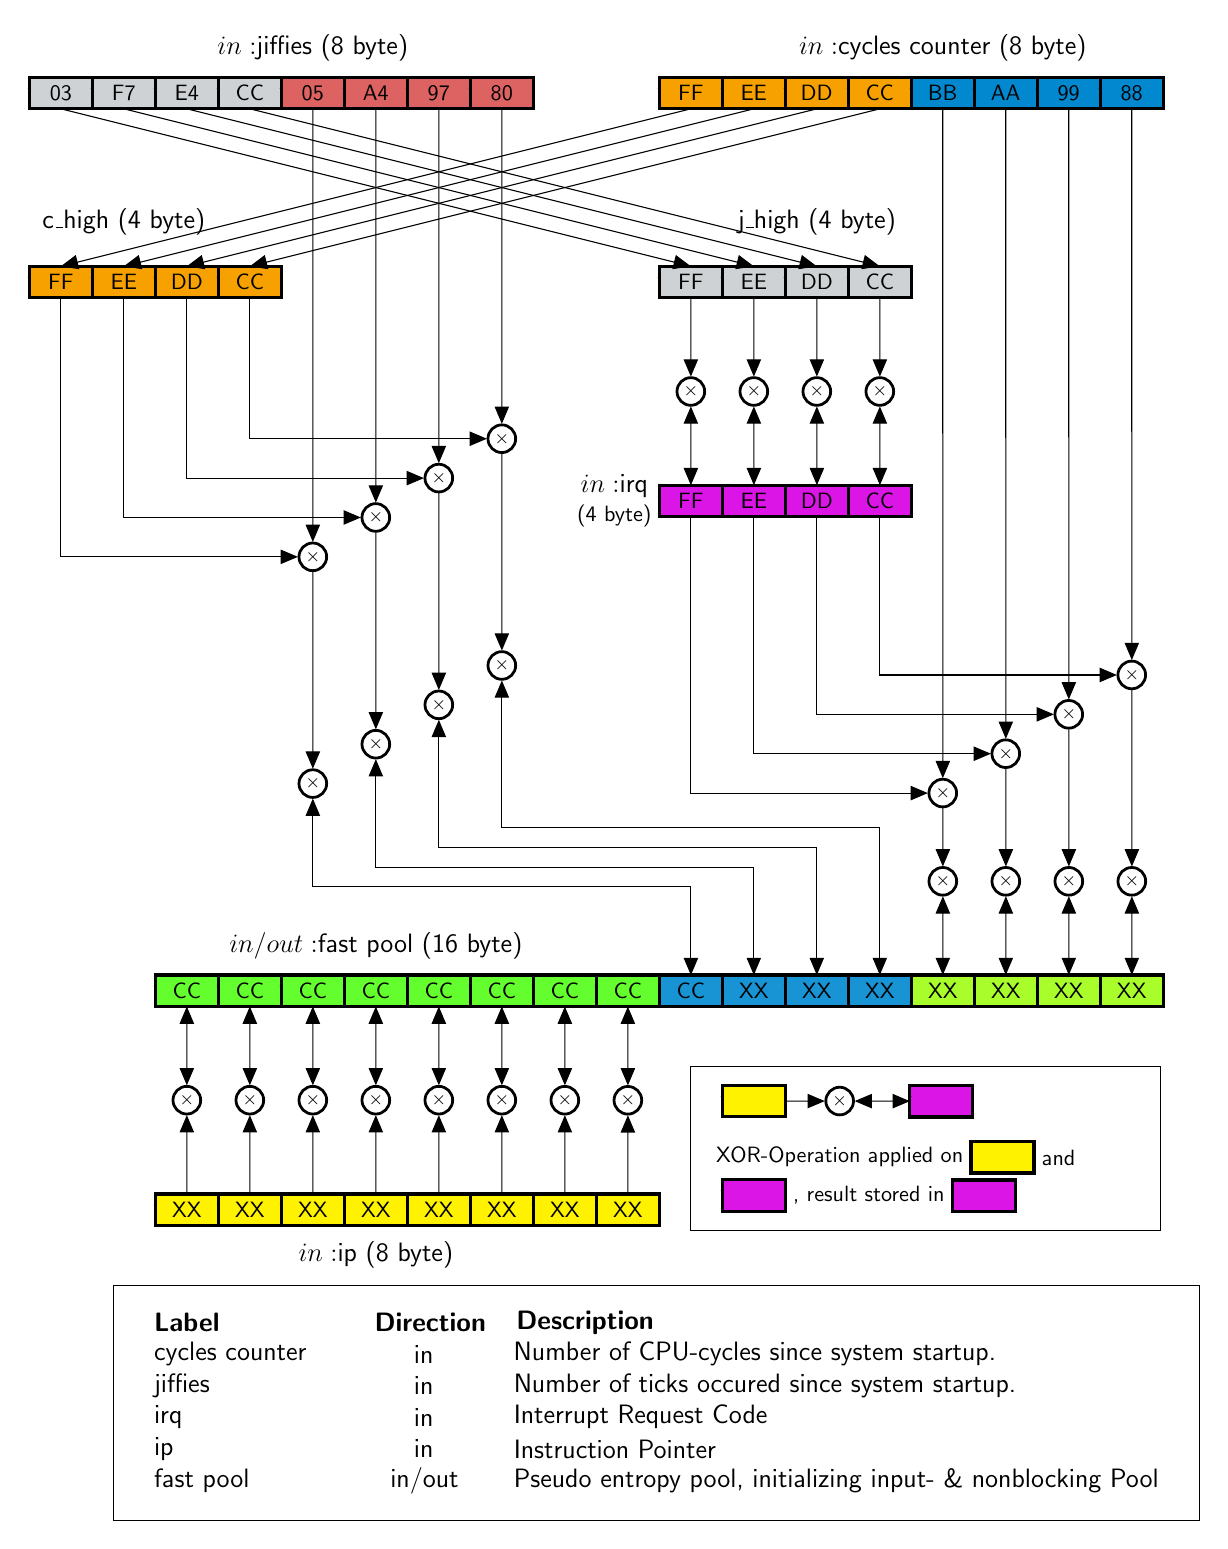
\begin{tikzpicture}[scale=0.8, every node/.style={scale=0.8},font=\sffamily,>=triangle 45]
	\tikzstyle{sum} = [draw, shape=circle, node distance=1.5cm, line width=1pt, minimum width=1.25em]	
	%\Huge
	\def\N{7}  % Number of Flip-Flops minus one
	\def\BW{1.8} % Byte Width

	% colors
	\definecolor{cjh}{HTML}{CFD2D4}
	\definecolor{cjl}{HTML}{DD6262}
	\definecolor{cch}{HTML}{F7A100}
	\definecolor{ccl}{HTML}{0288CF}
	\definecolor{cep32}{HTML}{64FE2E}
	\definecolor{cep1}{HTML}{1893D4}
	\definecolor{cep0}{HTML}{A9FD2A}
	\definecolor{cirq}{HTML}{DB15E5}
	\definecolor{cip}{HTML}{FFF200}

	% jiffies
	\node [shape=dff,fill=cjh] (jiff7) at ($ 1.0*(0,0) $) {03};
	\node [shape=dff,fill=cjh] (jiff6) at ($ 1.0*(1,0) $) {F7};
	\node [shape=dff,fill=cjh] (jiff5) at ($ 1.0*(2,0) $) {E4};
	\node [shape=dff,fill=cjh] (jiff4) at ($ 1.0*(3,0) $) {CC};			
	\node [shape=dff,fill=cjl] (jiff3) at ($ 1.0*(4,0) $) {05};
	\node [shape=dff,fill=cjl] (jiff2) at ($ 1.0*(5,0) $) {A4};
	\node [shape=dff,fill=cjl] (jiff1) at ($ 1.0*(6,0) $) {97};
	\node [shape=dff,fill=cjl] (jiff0) at ($ 1.0*(7,0) $) {80};	
	\node[above=1mm of jiff3] (ljiffies) {\large $in:$jiffies (8 byte)};		

	% jiffies low XOR c_high - XOR nodes
	\node [sum, below=4.0cm of jiff0, draw] (xjlch0) {};
	\node [sum, below=4.5cm of jiff1, draw] (xjlch1) {};	
	\node [sum, below=5.0cm of jiff2, draw] (xjlch2) {};
	\node [sum, below=5.5cm of jiff3, draw] (xjlch3) {};	
	\node [rotate=45] at (xjlch0) (plus) {{\footnotesize$+$}};
	\node [rotate=45] at (xjlch1) (plus) {{\footnotesize$+$}};	
	\node [rotate=45] at (xjlch2) (plus) {{\footnotesize$+$}};
	\node [rotate=45] at (xjlch3) (plus) {{\footnotesize$+$}};
		
	% cycles
	\node [shape=dff,fill=cch] (cycl7) at ($ 1.0*(10,0) $) {FF};
	\node [shape=dff,fill=cch] (cycl6) at ($ 1.0*(11,0) $) {EE};
	\node [shape=dff,fill=cch] (cycl5) at ($ 1.0*(12,0) $) {DD};
	\node [shape=dff,fill=cch] (cycl4) at ($ 1.0*(13,0) $) {CC};			
	\node [shape=dff,fill=ccl] (cycl3) at ($ 1.0*(14,0) $) {BB};
	\node [shape=dff,fill=ccl] (cycl2) at ($ 1.0*(15,0) $) {AA};
	\node [shape=dff,fill=ccl] (cycl1) at ($ 1.0*(16,0) $) {99};
	\node [shape=dff,fill=ccl] (cycl0) at ($ 1.0*(17,0) $) {88};
	\node[above=1mm of cycl3] (lcycles) {\large $in:$cycles counter (8 byte)};	

	%c_high
	\node [shape=dff,fill=cch, below=2cm of jiff7, draw] (chigh3) {FF};
	\node [shape=dff,fill=cch, below=2cm of jiff6, draw] (chigh2) {EE};
	\node [shape=dff,fill=cch, below=2cm of jiff5, draw] (chigh1) {DD};
	\node [shape=dff,fill=cch, below=2cm of jiff4, draw] (chigh0) {CC};
	\node[above=3mm of chigh2] (lchigh) {\large c\_high (4 byte)};			

	%j_high
	\node [shape=dff,fill=cjh, below=2cm of cycl7, draw] (jiffh3) {FF};
	\node [shape=dff,fill=cjh, below=2cm of cycl6, draw] (jiffh2) {EE};
	\node [shape=dff,fill=cjh, below=2cm of cycl5, draw] (jiffh1) {DD};
	\node [shape=dff,fill=cjh, below=2cm of cycl4, draw] (jiffh0) {CC};
	\node[above=3mm of jiffh1] (ljhigh) {\large j\_high (4 byte)};			

	% jiffies high XOR irq - XOR nodes
	\node [sum, below=1.0cm of jiffh3, draw] (xjhi3) {};	
	\node [rotate=45] at (xjhi3) (plus) {{\footnotesize$+$}};
	\node [sum, below=1.0cm of jiffh2, draw] (xjhi2) {};	
	\node [rotate=45] at (xjhi2) (plus) {{\footnotesize$+$}};
	\node [sum, below=1.0cm of jiffh1, draw] (xjhi1) {};	
	\node [rotate=45] at (xjhi1) (plus) {{\footnotesize$+$}};
	\node [sum, below=1.0cm of jiffh0, draw] (xjhi0) {};	
	\node [rotate=45] at (xjhi0) (plus) {{\footnotesize$+$}};
			
	%irq
	\node [shape=dff,fill=cirq, below=1cm of xjhi3, draw] (irq3) {FF};
	\node [shape=dff,fill=cirq, below=1cm of xjhi2, draw] (irq2) {EE};
	\node [shape=dff,fill=cirq, below=1cm of xjhi1, draw] (irq1) {DD};
	\node [shape=dff,fill=cirq, below=1cm of xjhi0, draw] (irq0) {CC};
	\node[left=0mm of irq3] (lirq) {\shortstack{\large $in:$irq\\(4 byte)}};	
	
	% cycles low XOR irq - XOR nodes
	\node [sum, below=8.5cm of cycl3, draw] (xcli3) {};
	\node [sum, below=8.0cm of cycl2, draw] (xcli2) {};	
	\node [sum, below=7.5cm of cycl1, draw] (xcli1) {};		
	\node [sum, below=7.0cm of cycl0, draw] (xcli0) {};			
	\node [rotate=45] at (xcli3) (plus) {{\footnotesize$+$}};
	\node [rotate=45] at (xcli2) (plus) {{\footnotesize$+$}};	
	\node [rotate=45] at (xcli1) (plus) {{\footnotesize$+$}};
	\node [rotate=45] at (xcli0) (plus) {{\footnotesize$+$}};	
	
	% entropy pool	
	\node [shape=dff,fill=cep32, below=11cm of jiff5, draw] (entp15) {CC};		
	\node [shape=dff,fill=cep32, below=11cm of jiff4, draw] (entp14) {CC};
	\node [shape=dff,fill=cep32, below=11cm of jiff3, draw] (entp13) {CC};
	\node [shape=dff,fill=cep32, below=11cm of jiff2, draw] (entp12) {CC};
	\node [shape=dff,fill=cep32, below=11cm of jiff1, draw] (entp11) {CC};
	\node [shape=dff,fill=cep32, below=11cm of jiff0, draw] (entp10) {CC};
	\node [shape=dff,fill=cep32, right=0cm of entp10, draw] (entp9) {CC};	
	\node [shape=dff,fill=cep32, right=0cm of entp9, draw] (entp8) {CC};
	\node [shape=dff,fill=cep1, right=0cm of entp8, draw] (entp7) {CC};
	\node [shape=dff,fill=cep1, below=11cm of cycl6, draw] (entp6) {XX};	
	\node [shape=dff,fill=cep1, below=11cm of cycl5, draw] (entp5) {XX};	
	\node [shape=dff,fill=cep1, below=11cm of cycl4, draw] (entp4) {XX};	
	\node [shape=dff,fill=cep0, below=11cm of cycl3, draw] (entp3) {XX};	
	\node [shape=dff,fill=cep0, below=11cm of cycl2, draw] (entp2) {XX};	
	\node [shape=dff,fill=cep0, below=11cm of cycl1, draw] (entp1) {XX};	
	\node [shape=dff,fill=cep0, below=11cm of cycl0, draw] (entp0) {XX};	
	\node[above=1mm of entp12] (lentp) {\large $in/out:$fast pool (16 byte)};	

	%% XOR entp
	% ch / jl 
	\node [sum, below=2.5cm of xjlch3, draw] (xentp7) {};	
	\node [rotate=45] at (xentp7) (plus) {{\footnotesize$+$}};
	\node [sum, below=2.5cm of xjlch2, draw] (xentp6) {};	
	\node [rotate=45] at (xentp6) (plus) {{\footnotesize$+$}};
	\node [sum, below=2.5cm of xjlch1, draw] (xentp5) {};	
	\node [rotate=45] at (xentp5) (plus) {{\footnotesize$+$}};
	\node [sum, below=2.5cm of xjlch0, draw] (xentp4) {};	
	\node [rotate=45] at (xentp4) (plus) {{\footnotesize$+$}};									
	% irq/cycl 
	\node [sum, above=1.0cm of entp3, draw] (xentp3) {};	
	\node [rotate=45] at (xentp3) (plus) {{\footnotesize$+$}};
	\node [sum, above=1.0cm of entp2, draw] (xentp2) {};	
	\node [rotate=45] at (xentp2) (plus) {{\footnotesize$+$}};
	\node [sum, above=1.0cm of entp1, draw] (xentp1) {};	
	\node [rotate=45] at (xentp1) (plus) {{\footnotesize$+$}};
	\node [sum, above=1.0cm of entp0, draw] (xentp0) {};	
	\node [rotate=45] at (xentp0) (plus) {{\footnotesize$+$}};		
	% ip
	\node [sum, below=1.0cm of entp15, draw] (xentp15) {};	
	\node [rotate=45] at (xentp15) (plus) {{\footnotesize$+$}};
	\node [sum, below=1.0cm of entp14, draw] (xentp14) {};	
	\node [rotate=45] at (xentp14) (plus) {{\footnotesize$+$}};
	\node [sum, below=1.0cm of entp13, draw] (xentp13) {};	
	\node [rotate=45] at (xentp13) (plus) {{\footnotesize$+$}};
	\node [sum, below=1.0cm of entp12, draw] (xentp12) {};	
	\node [rotate=45] at (xentp12) (plus) {{\footnotesize$+$}};		
	\node [sum, below=1.0cm of entp11, draw] (xentp11) {};	
	\node [rotate=45] at (xentp11) (plus) {{\footnotesize$+$}};
	\node [sum, below=1.0cm of entp10, draw] (xentp10) {};	
	\node [rotate=45] at (xentp10) (plus) {{\footnotesize$+$}};
	\node [sum, below=1.0cm of entp9, draw] (xentp9) {};	
	\node [rotate=45] at (xentp9) (plus) {{\footnotesize$+$}};
	\node [sum, below=1.0cm of entp8, draw] (xentp8) {};	
	\node [rotate=45] at (xentp8) (plus) {{\footnotesize$+$}};	

	\node [shape=dff,fill=cip, below=1cm of xentp15, draw] (ip7) {XX};	
	\node [shape=dff,fill=cip, below=1cm of xentp14, draw] (ip6) {XX};
	\node [shape=dff,fill=cip, below=1cm of xentp13, draw] (ip5) {XX};
	\node [shape=dff,fill=cip, below=1cm of xentp12, draw] (ip4) {XX};
	\node [shape=dff,fill=cip, below=1cm of xentp11, draw] (ip3) {XX};
	\node [shape=dff,fill=cip, below=1cm of xentp10, draw] (ip2) {XX};
	\node [shape=dff,fill=cip, below=1cm of xentp9, draw] (ip1) {XX};
	\node [shape=dff,fill=cip, below=1cm of xentp8, draw] (ip0) {XX};
	\node[below=1mm of ip4] (lip) {\large $in:$ip (8 byte)};	

	%%%%%% LINES >>
	
	% jiffies  -> c_low - lines
	\draw [->] (jiff3.south) -- (xjlch3.north);
	\draw [->] (jiff2.south) -- (xjlch2.north);	
	\draw [->] (jiff1.south) -- (xjlch1.north);		
	\draw [->] (jiff0.south) -- (xjlch0.north);		

	% c_high -> xjlch
	\draw [->] (chigh3.south)|- (xjlch3.west);
	\draw [->] (chigh2.south)|- (xjlch2.west);
	\draw [->] (chigh1.south)|- (xjlch1.west);
	\draw [->] (chigh0.south)|- (xjlch0.west);			

	% jiffies high -> j_high
	\draw [->] (jiff7.south) -- (jiffh3.north);
	\draw [->] (jiff6.south) -- (jiffh2.north);	
	\draw [->] (jiff5.south) -- (jiffh1.north);		
	\draw [->] (jiff4.south) -- (jiffh0.north);		

	% cycles_high -> c_high
	\draw [->] (cycl7.south) -- (chigh3.north);
	\draw [->] (cycl6.south) -- (chigh2.north);	
	\draw [->] (cycl5.south) -- (chigh1.north);		
	\draw [->] (cycl4.south) -- (chigh0.north);		
	
	% cycles_low -> c_high
	\draw [->] (cycl3.south) -- (xcli3.north);
	\draw [->] (cycl2.south) -- (xcli2.north);	
	\draw [->] (cycl1.south) -- (xcli1.north);		
	\draw [->] (cycl0.south) -- (xcli0.north);	

	% jiffies high -> j_high
	\draw [->] (jiffh3.south) -- (xjhi3.north);
	\draw [->] (jiffh2.south) -- (xjhi2.north);	
	\draw [->] (jiffh1.south) -- (xjhi1.north);		
	\draw [->] (jiffh0.south) -- (xjhi0.north);
		
	% xjhi -> irq
	\draw [<->] (xjhi3.south) -- (irq3.north);
	\draw [<->] (xjhi2.south) -- (irq2.north);	
	\draw [<->] (xjhi1.south) -- (irq1.north);		
	\draw [<->] (xjhi0.south) -- (irq0.north);
	
	% xjlch -> xentp
	\draw [->] (xjlch3.south) -- (xentp7.north);
	\draw [->] (xjlch2.south) -- (xentp6.north);	
	\draw [->] (xjlch1.south) -- (xentp5.north);		
	\draw [->] (xjlch0.south) -- (xentp4.north);

	% irq -> xcli
	\draw [->] (irq3.south) |- (xcli3.west);
	\draw [->] (irq2.south) |- (xcli2.west);	
	\draw [->] (irq1.south) |- (xcli1.west);		
	\draw [->] (irq0.south) |- (xcli0.west);

	% xentp -> entp
	\draw [<->] (xentp7.south) |- ($(entp7.north)!1/2!(entp7.north |- xentp7.south)$) coordinate (C1) -| (entp7.north);			
	\draw [<->] (xentp6.south) |- ($(entp6.north)!1/2!(entp6.north |- xentp6.south)$) coordinate (C2) -| (entp6.north);		
	\draw [<->] (xentp5.south) |- ($(entp5.north)!1/2!(entp5.north |- xentp5.south)$) coordinate (C3) -| (entp5.north);				
	\draw [<->] (xentp4.south) |- ($(entp4.north)!1/2!(entp4.north |- xentp4.south)$) coordinate (C4) -| (entp4.north);	
	
	% xcli -> xentp
	\draw [->] (xcli3.south) -- (xentp3.north);
	\draw [->] (xcli2.south) -- (xentp2.north);	
	\draw [->] (xcli1.south) -- (xentp1.north);		
	\draw [->] (xcli0.south) -- (xentp0.north);	

	% xcli -> xentp
	\draw [<->] (xentp3.south) -- (entp3.north);
	\draw [<->] (xentp2.south) -- (entp2.north);	
	\draw [<->] (xentp1.south) -- (entp1.north);		
	\draw [<->] (xentp0.south) -- (entp0.north);
	
	% xentp -> entp
	\draw [<->] (xentp15.north) -- (entp15.south);
	\draw [<->] (xentp14.north) -- (entp14.south);
	\draw [<->] (xentp13.north) -- (entp13.south);
	\draw [<->] (xentp12.north) -- (entp12.south);
	\draw [<->] (xentp11.north) -- (entp11.south);
	\draw [<->] (xentp10.north) -- (entp10.south);
	\draw [<->] (xentp9.north) -- (entp9.south);
	\draw [<->] (xentp8.north) -- (entp8.south);
	
	% ip -> xentp
	\draw [->] (ip7.north) -- (xentp15.south);
	\draw [->] (ip6.north) -- (xentp14.south);
	\draw [->] (ip5.north) -- (xentp13.south);
	\draw [->] (ip4.north) -- (xentp12.south);
	\draw [->] (ip3.north) -- (xentp11.south);
	\draw [->] (ip2.north) -- (xentp10.south);
	\draw [->] (ip1.north) -- (xentp9.south);
	\draw [->] (ip0.north) -- (xentp8.south);
	
	%%%%%% Legende 
\begin{scope}
	\node [shape=dff,fill=cip, below=10mm of entp6, draw] (f8) {};
	\node [sum, right=5mm of f8, draw] (xf8) {};	
	\node [rotate=45] at (xf8) (plus) {{\footnotesize$+$}};	
	\node [shape=dff,fill=cirq, right=7mm of xf8, draw] (c3) {};
	\draw [->] (f8.east) -- (xf8.west);
	\draw [<->] (xf8.east) -- (c3.west);
	\node[black, below=3mm of xf8, align=left] (lf81) {XOR-Operation applied on};	
	\node [shape=dff,fill=cip, right=0mm of lf81, draw] (rf8) {};
	\node[black, right=0mm of rf8, align=left] (lf82) {and};	
	
	\node [shape=dff,fill=cirq, below=22mm of entp6, draw] (yf8) {};
	\node[black, right=0mm of yf8, align=left] (lf83) {, result stored in};
	\node [shape=dff,fill=cirq, right=0mm of lf83, draw] (zf8) {};	
	\draw[black] ([xshift=-5mm, yshift=3mm ]f8.north west) rectangle ([xshift=23mm, yshift=-3mm]zf8.south east);	
\end{scope}	

\begin{scope}
\large
%\node [draw, align=center] {Text\\und Text};
\node[black, below=10mm of ip7, align=left] (lghdlbl) {\textbf{Label}};	
\node[black, right=28mm of lghdlbl.west, anchor=west, align=left] (lghddirr) {\textbf{Direction}};
\node[black, right=18mm of  lghddirr.west, anchor=west, align=left] (lghddesc) {\textbf{Description}};

%\node[black, below=10mm of ip4, align=left] (lgjif) {\textbf{cycles counter}};	
\node[black, below=4mm of lghdlbl.west, anchor=west, align=left] (lgcc) {cycles counter};	
\node[black, below=4mm of lgcc.west, anchor=west] (lgjif) {jiffies};	
\node[black, below=4mm of lgjif.west, anchor=west] (lgirq) {irq};	
\node[black, below=4mm of lgirq.west, anchor=west] (lgip) {ip};
\node[black, below=4mm of lgip.west, anchor=west] (lgentp) {fast pool};

\node[black, right=33mm of lgcc.west, align=left] (lgdircc) {in};	
\node[black, right=33mm of lgjif.west, align=left] (lgdirjif) {in};	
\node[black, right=33mm of lgirq.west, align=left] (lgdirirq) {in};
\node[black, right=33mm of lgip.west, align=left] (lgdirip) {in};
\node[black, right=30mm of lgentp.west, align=center] (lgdientp) {in/out};


\node[black, right=24mm of lgcc, align=left] (lgcctxt) {Number of CPU-cycles since system startup.};	
\node[black, below=4mm of lgcctxt.west, anchor=west] (lgjiftxt) {Number of ticks occured since system startup.};	
\node[black, below=4mm of lgjiftxt.west, anchor=west] (lgirqtxt) {Interrupt Request Code};
\node[black, below=4mm of lgirqtxt.west, anchor=west] (lgiptxt) {Instruction Pointer};
\node[black, below=4mm of lgiptxt.west, anchor=west] (lgentptxt) {Pseudo entropy pool, initializing input- \& nonblocking Pool};

\draw[black] ([xshift=-5mm, yshift=3mm ]lghdlbl.north west) rectangle ([xshift=5mm, yshift=-3mm]lgentptxt.south east);
	
\end{scope}
\end{tikzpicture}
\caption{Pre-processing of input parameters by function 'add\_interrupt\_randomness' before applying further operations via fast\_mix / mix\_pool\_bytes (valid for x64 / 64-bit Kernel only)} \label{fig:add-int-rnd}
\end{figure}

\begin{figure}[H]
	\centering
	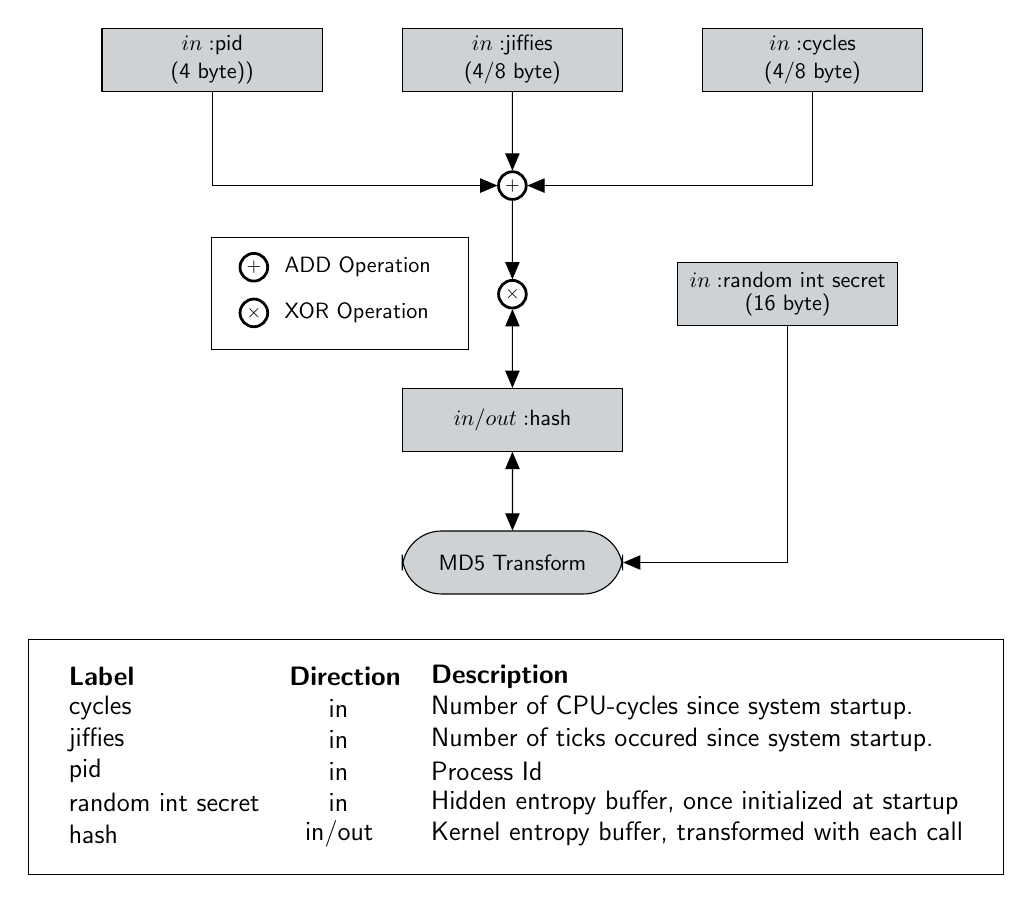
\begin{tikzpicture}[scale=0.8, every node/.style={scale=0.8},font=\sffamily,>=triangle 45]
	\tikzstyle{sum} = [draw, shape=circle, node distance=1.5cm, line width=1pt, minimum width=1.25em]	
	%\Huge
	\def\N{7}  % Number of Flip-Flops minus one
	\def\BW{1.8} % Byte Width
	
	% colors
	\definecolor{cjh}{HTML}{CFD2D4}
	\definecolor{cjl}{HTML}{DD6262}
	\definecolor{cch}{HTML}{F7A100}
	\definecolor{ccl}{HTML}{0288CF}
	\definecolor{cep32}{HTML}{64FE2E}
	\definecolor{cep1}{HTML}{1893D4}
	\definecolor{cep0}{HTML}{A9FD2A}
	\definecolor{cirq}{HTML}{DB15E5}
	\definecolor{cip}{HTML}{FFF200}
	
	% rect rc-inp-pid
	\node (rc-inp-pid) [rectangle, fill=cjh, draw, minimum width=35mm, minimum height=10mm, anchor= south west] at (0,0) {\shortstack{$in:$pid\\(4 byte))}};
	% rect rc-inp-jiffies
	\node (rc-inp-jiffies) [rectangle, right=10mm of rc-inp-pid, fill=cjh, draw, minimum width=35mm, minimum height=10mm, anchor= west] {\shortstack{$in:$jiffies\\(4/8 byte)}};	
	% rect rc-inp-cycles	
	\node (rc-inp-cycles) [rectangle, right=10mm of rc-inp-jiffies, fill=cjh, draw, minimum width=35mm, minimum height=10mm, anchor= west] {\shortstack{$in:$cycles\\(4/8 byte)}};	
	% oa-pjc - add pid/jiffies/cycles
	\node [sum, below=10mm of rc-inp-jiffies, draw] (oa-pjc) {};	
	\node at (oa-pjc) (plus) {{\footnotesize$+$}};	
	% rc-inp-pid -> oa-pjc
	\draw [->] (rc-inp-pid) |- (oa-pjc);	
	% rc-inp-jiffies -> oa-pjc
	\draw [->] (rc-inp-jiffies) -- (oa-pjc);
	% rc-inp-cycles -> oa-pjc
	\draw [->] (rc-inp-cycles) |- (oa-pjc);
	% ox-oa-pjc-hash 
	\node [sum, below=10mm of oa-pjc, draw] (ox-oa-pjc-hash) {};	
	\node [rotate=45] at (ox-oa-pjc-hash) (plus) {{\footnotesize$+$}};	
	% oa-pjc -> ox-oa-pjc-hash
	\draw [->] (oa-pjc) -- (ox-oa-pjc-hash);	
	% rc-hash	
	\node (rc-hash) [rectangle, below=10mm of ox-oa-pjc-hash, fill=cjh, draw, minimum width=35mm, minimum height=10mm] {\shortstack{$in/out:$hash}};		
	% ox-oa-pjc-hash <-> md5-transf
	\draw [<->] (ox-oa-pjc-hash) -- (rc-hash);	
	% md5-transf
	\node (md5-transf) [rectangle, below=10mm of rc-hash, fill=cjh, draw, minimum width=35mm, minimum height=10mm, rounded corners=0.5cm] {\shortstack{MD5 Transform}};	
	% rc-hash <-> md5-transf
	\draw [<->] (rc-hash) -- (md5-transf);
	% rect rc-rnd-int-sec
	\node (rc-rnd-int-sec) [rectangle, right=19mm of ox-oa-pjc-hash, fill=cjh, draw, minimum width=35mm, minimum height=10mm, anchor= west] {\shortstack{$in:$random int secret\\(16 byte)}};	
	% rc-rnd-int-sec <-> md5-transf
	\draw [->] (rc-rnd-int-sec) |- (md5-transf);
	
	%%%%%%%%% Legende
	\begin{scope}
	
	% ox
	\node [sum,  below right=25mm and 18mm of rc-inp-pid.west, draw] (loa) {};	
	\node at (loa) (plus) {{\footnotesize$+$}};	
	\node[black, right=1mm of loa.east, anchor=west, align=left] (lloa) {ADD Operation};		
	% oa
	\node [sum, below=2mm of loa, draw] (lox) {};	
	\node [rotate=45] at (lox) (plus) {{\footnotesize$+$}};	
	\node[black, right=1mm of lox.east, anchor=west, align=left] (llox) {XOR Operation};		

	\draw[black] ([xshift=-5mm, yshift=3mm ]loa.north west) rectangle ([xshift=5mm, yshift=-3mm]llox.south east);	
	
	\end{scope}
		
	\begin{scope}	
	\large
	%\node [draw, align=center] {Text\\und Text};
	\node[black, below=76mm of rc-inp-pid.west, align=left] (lghdlbl) {\textbf{Label}};	
	\node[black, right=28mm of lghdlbl.west, anchor=west, align=left] (lghddirr) {\textbf{Direction}};
	\node[black, right=18mm of  lghddirr.west, anchor=west, align=left] (lghddesc) {\textbf{Description}};
	
	%\node[black, below=10mm of ip4, align=left] (lgjif) {\textbf{cycles counter}};	
	\node[black, below=4mm of lghdlbl.west, anchor=west, align=left] (lgcc) {cycles};	
	\node[black, below=4mm of lgcc.west, anchor=west] (lgjif) {jiffies};	
	\node[black, below=4mm of lgjif.west, anchor=west] (lgirq) {pid};	
	\node[black, below=4mm of lgirq.west, anchor=west] (lgip) {random int secret};
	\node[black, below=4mm of lgip.west, anchor=west] (lgentp) {hash};
	
	\node[black, right=33mm of lgcc.west, align=left] (lgdircc) {in};	
	\node[black, right=33mm of lgjif.west, align=left] (lgdirjif) {in};	
	\node[black, right=33mm of lgirq.west, align=left] (lgdirirq) {in};
	\node[black, right=33mm of lgip.west, align=left] (lgdirip) {in};
	\node[black, right=30mm of lgentp.west, align=center] (lgdientp) {in/out};
	
	
	\node[black, right=46mm of lgcc.west, align=left] (lgcctxt) {Number of CPU-cycles since system startup.};	
	\node[black, below=4mm of lgcctxt.west, anchor=west] (lgjiftxt) {Number of ticks occured since system startup.};	
	\node[black, below=4mm of lgjiftxt.west, anchor=west] (lgirqtxt) {Process Id};
	\node[black, below=4mm of lgirqtxt.west, anchor=west] (lgiptxt) {Hidden entropy buffer, once initialized at startup};
	\node[black, below=4mm of lgiptxt.west, anchor=west] (lgentptxt) {Kernel entropy buffer, transformed with each call};
	
	\draw[black] ([xshift=-5mm, yshift=3mm ]lghdlbl.north west) rectangle ([xshift=5mm, yshift=-3mm]lgentptxt.south east);
	
	\end{scope}	

\end{tikzpicture}	
	\caption{Processing of input parameters by function 'get\_random\_int/long' (valid for x64 / 64-bit Kernel only)} \label{fig:get-rnd-int-long}
\end{figure}



%\begin{mdframed}
%\begin{tabularx}{\columnwidth}{XXl}
%\begin{tabularx}{\textwidth}{ll}
%%	\caption{Description of input parameters proccessed by func. 'add\_interrupt\_randomness'}
%%	\label{tab:add-int-rnd-desc}\\
%	\textbf{jiffies}&Igel\\
%	\textbf{cycles counter}&Dienstag\\
%	\textbf{irq}&\\
%	\textbf{ip}&\textit{Instruction Pointer}
%	\caption{Description of input parameters proccessed by func. 'add\_interrupt\_randomness'}
%\end{tabularx}
%\centering
%\begin{table}[H]
%	\begin{tabular}{ll}
%	\textbf{Jiffies}&Nr. of ticks occured since system startup.\\
%	\textbf{Cycles Counter}&Nr. of CPU-cycles since system startup.\\
%	\textbf{irq}&Interrupt Request \\
%	\textbf{ip}&\textit{Instruction Pointer}
%	\end{tabular}
%	\caption{Description of input parameters proccessed by func. 'add\_interrupt\_randomness'}	
%\end{table}

% jiffies . Incremented for each timer interrupt.
% . also known as \textit{Time Stamp Counter}.

%	\cite{kernlrandmc}
		
%\end{mdframed}


%\begin{tabularx}{\columnwidth}{XXl}
%	jiffies&Schnecke&Igel\\
%	cycles counter&Hier ist ein langes Wort Hier ist ein langes Wort Hier ist ein langes Wort Hier ist ein langes Wort &Dienstag\\
%	irq&&\\
%	ip&&
%\end{tabularx}
%
%
%
%\begin{mdframed}
%\begin{description}
%	\item [jiffies] sadfasdfsadf
%	\item [cycles counter] asdfasdfasdf
%	\item [irq] asdfasdfasdf	
%	\item [ip] 
%\end{description}
%\cite{kernlrandmc}	
%\end{mdframed}




\section{Conclusion}
The final section of the chapter gives an overview of the important results
of this chapter. This implies that the introductory chapter and the
concluding chapter don't need a conclusion.

%\lipsum[66]

%%% Local Variables: 
%%% mode: latex
%%% TeX-master: "thesis"
%%% End: 

\chapter{NIST Special Publication 800-90B}
\label{chap:NIST800-90B}
\section{General}

Topic of this thesis is an analysis of a Linux Random Number Generator's outcome delivered to kernel consumers, as introduced in \ref{sub:get-rnd-int-long}. Verification and estimation of entropy is 
a very difficult task, since there is no explicit definition for randomness. Hence, for a series of values generated by an RNG, randomness i.e. a sufficient degree of entropy is admitted, if the absence of any discernible pattern within a generated record can be diagnosed.
To assess the outcome and reliability of random number generating devices or implementations, several frameworks have been published, providing recommendations regarding the solid construction and validation of PRNG and TRNG sources. These also encompass a set of statistical tests and guidance how to conduct a profound verification (see \cite{robert2006dieharder, rukhin2010nist, turan2018nist}).
The National Institute of Standards and Technology (NIST) publishes a series of documents that describe U.S. federal government computer security policies, procedures and guidelines called NIST 800 series (see \cite[]{nist800pub}). To implement the analysis of this thesis, two Special Publications on the subject of validation and assessment of entropy and random number generation has been chosen:

\begin{table}[H]
	\centering
	\label{tab:nist800sps}
	\begin{tabular}{lll}\\ \hline 
		Number & Title & Release Date \\ \hline \hline 
		800-90B & \makecell[l]{Recommendation for the Entropy Sources Used for\\Random Bit Generation} & 1/10/2018 \\ \hline 
		800-22 Rev. 1a & \makecell[l]{A Statistical Test Suite for Random and Pseudorandom\\Number Generators for Cryptographic Applications} & 4/30/2010 \\ \hline 
	\end{tabular}
	\caption{Applied NIST Special Publications of the 800 Series (Status Final)}
\end{table} 


For this analysis, a framework based on 'Recommendation for the Entropy Sources Used for Random Bit Generation, NIST Special Publication 800- 90B' \cite{turan2018nist} has been chosen, able to deliver
usable guidance that will give conservative estimates on the amount of entropy in an entropy
source \cite{turan2015random}. The final version of the framework has been published in january 2018 and thus is very up to date. Beside that this decision has been met, since not just the outcome of and RNG can be assessed but also it's input. As mentioned in \ref{sec:int-rnd}, the Linux RNG executed on a Xen virtualized machine is not able to obtain noise from most designated sources. In fact, interrupt noise is the only input delivered during the initialization phase. Hence, to achieve a comprehensive analysis, an assessment of this input is considered to be required.\\
'NIST Special Publication (SP) 800-90' (a series consisting of three documents) specifies how to design an test 

 is all about
generating random numbers for cryptography. In SP 800-90, this is a two-stage process: first, an
entropy source provides an impossible-to-guess seed. Then, a deterministic cryptographic
algorithm (called a DRBG--deterministic random bit generator--in SP 800-90) expands the seed
into a long sequence of values that may be safely used for keys, IVs, nonces, etc.
\cite{turan2015random}.



 When assessing entropy by the second part of the series, 'NIST Special Publication 800-90B' (in the following referred to as NSP800-90B), an estimation can be achieved via 
two different tracks. Depending on an assumption regarding an entropy source, which has to be substantiated, the IID i.e. the Non-IID track should be used to analyze assumed random input 
\cite{turan2018nist}. The outcome of an analysis is an estimation of entropy, ascertained by statistical tests expressed in \textit{bits of entropy}. In the following sections, an introduction to these procedures, required to comprehend the results in TODO[Evaludation] is given.



%-----------------------------------------------
%NIST Special Publication (SP) 800-90 (a series consisting of three documents) is all about
%generating random numbers for cryptography. In SP 800-90, this is a two-stage process: first, an
%entropy source provides an impossible-to-guess seed. Then, a deterministic cryptographic
%algorithm (called a DRBG--deterministic random bit generator--in SP 800-90) expands the seed
%into a long sequence of values that may be safely used for keys, IVs, nonces, etc.
%\cite{turan2015random}

\section{Definitions \& Terminology}

\subsection{Distinction: Noise / Entropy / Randomness / RNG}
In literature, terms describing the in- and output of RNGs are sometimes used in a generic and partially confusing manner. For this thesis, the following terminology will be used, intending to distinguish regarding the maturity, source and purpose of (pseudo) random numbers.

\begin{itemize}
	\item \textbf{Entropy} Entropy is a property of a variable or value describing a certain degree of unpredictability. 
	\item \textbf{Noise} Noise is the input passed to an RNG or and intermediate processing stage.
	While there might be a wide range, in general, noise is not assumed to provide a cryptographic safe degree of entropy. Since the Linux RNG enriches entropy via various steps (see \ref{fig:linux-prng-arch}) depending on the stage \textit{Noise} will be subdivided into:
	\begin{itemize}
		\item \textbf{Raw Noise} Noise sources of the Linux RNG, delivering external physical states like interrupts (see \ref{sec:inp-src-lprng}).
		\item \textbf{Pre-processed Noise} Raw Noise being pre-processed via the fast-pool, assumed to have a poor level of entropy (see \ref{sub:fast-pool}).
		\item \textbf{Conditioned Noise} Noise prepared by a conditioning component and hence providing an advanced level of entropy, like the input-pool (see \ref{sub:input-pool}).	
	\end{itemize}
	\item \textbf{Randomness} The outcome of an RNG delivered to a user mode or kernel consumer. This output is assumed to provide a cryptographic safe degree of entropy.
	\item \textbf{Entropy Source} The generic term for any kind of sources dedicated to deliver values assumed to provide a certain degree of entropy. This includes all kind of \textit{Noise Sources} as well as \textit{Randomness Sources}.	
	\item \textbf{RBG/RNG} NIST 800 uses the more generalizing term \textit{RBG (Random Bit Generator)} instead of \textit{RNG (Random Number Generator)}. Since this thesis relates to Linux x86 Kernel where random numbers are always obtained and applied on at least byte level \textit{RNG} will used.
\end{itemize}

\subsection{The Definition of Entropy}
In Information theory, for a set of information units, entropy in generall describes the level of disorder i.e. the unpredictability of each single unit's state at a given alphabet. Various formal definitions of entropy exist \cite{hagerty2012entropy}, while the definition of Shannon (see \ref{fig:form-entropy-shan}) is quite common for a binary alphabet. 

\begin{figure}[H]
	\begin{align*}
	\displaystyle H(X) := \sum_{s \in {0,1}} I(p_s) p_s = \sum_{s \in {0,1}} -\lg_2 \frac{1}{p_s} p_s && \text{$p_s$ = P(X=s)}
	\end{align*}
	\caption{Formal definiton of entropy by Shannon for a binary alphabet}
	\label{fig:form-entropy-shan}
\end{figure}
According to Shannon, entropy is defined as the product of self-information \textit{I} multiplied by the expected value. For a binary alphabet, it can be measured in unit bits. 



\section{NIST Special Publication 800-90 B}

The NIST Special Publication (SP) 800-90 series of recommendations provides 
guidance on the validation and construction of Pseudo- and Non-deterministic Random Number Generators that can be used for cryptographic secure applications. More precisely the recommendation specifies how to design and validate entropy delivering sources that are be used as input i.e. for RNGs. Transfered to the Linux RNG this verification approach can be applied to the raw noise sources described in \ref{sec:inp-src-lprng} as well as conditioned input-pool or pre-processed noise of the  
fast-pool (\ref{sub:input-pool}, \ref{sub:fast-pool}). The series consist of three parts. NSP800-90A and NSP800-90C refer to the construction of RNG mechanisms, while NSP800-90B addresses the analysis and validation of sources delivering (prepared) noise. A source that conforms to this recommendation can be used by RNGs to produce a sequence of random values \cite{rukhin2010nist}.

\subsection{Min-Entropy}

\begin{equation}
	A = \{x_1, x_2, x_3, ..., x_k\}
	\label{eq:min-ent-A}
\end{equation}
\begin{equation}
	Pr(X=x_i) = p_i 
	\Domain{i=\{1,...,k\}}
\end{equation}
\begin{equation}
	H = \underset{1\leq i\leq k}{\mathrm{min}}(-\log_2p_i) = -\log_2 \underset{1\leq i\leq k}{\mathrm{max}}p_i
\end{equation}



\begin{figure}[H]
	\label{fig:entropy-est-strategy}
	\centering
	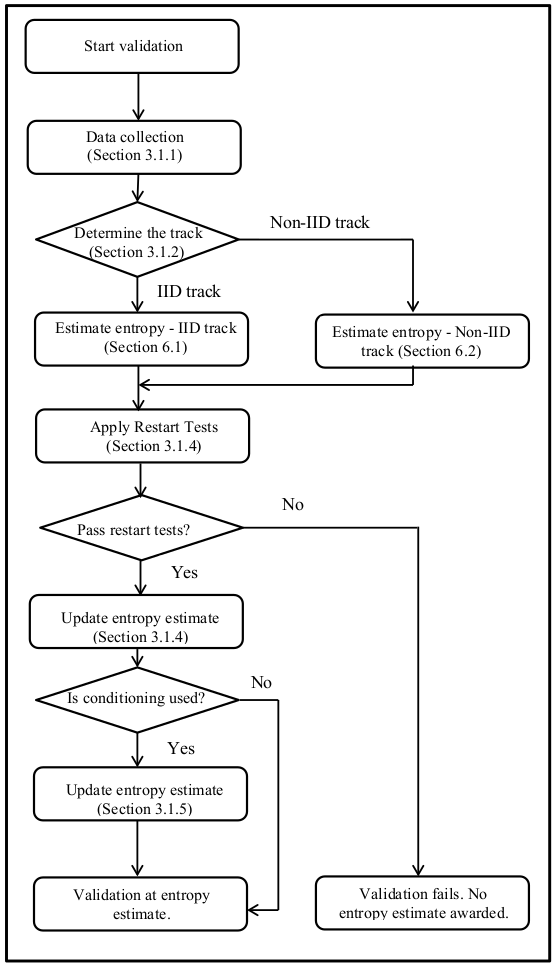
\includegraphics[scale=0.6]{img/nsp800-90b-entropy-est-strategy.png}
	\caption{Entropy Estimation Strategy according to NIST SP 800-90B (from \cite{turan2018nist}, references illustrated refer to the document)}
\end{figure}





\chapter{Experimental Setup \& Evaluation}
\label{chap:exp-setup-eavluation}

\input{tab-jiff-cycles-ip-v01.tex}


%  sudo xenstore-write "/local/domain/$xvuhv01_domu_id/bios-strings/system-manufacturer" "GSRN 2015 - MBA Thesis - Oliver Jessl"
%  sudo xenstore-write "/local/domain/$xvuhv01_domu_id/bios-strings/system-serial-number" "01234567-89ab-cdef-fedc-9876543210ff"
%  echo "modifying bios domain $xvuhv02_domu_id"
%  
%  sudo xenstore-write "/local/domain/$xvuhv02_domu_id/bios-strings/system-manufacturer" "GSRN 2015 - MBA Thesis - Oliver Jessl"
%  sudo xenstore-write "/local/domain/$xvuhv02_domu_id/bios-strings/system-serial-number" "01234567-89ab-cdef-fedc-9876543210ff"


\chapter{Security Components}
\label{chap:sec-components}


\begin{figure}[H]
	\centering
	    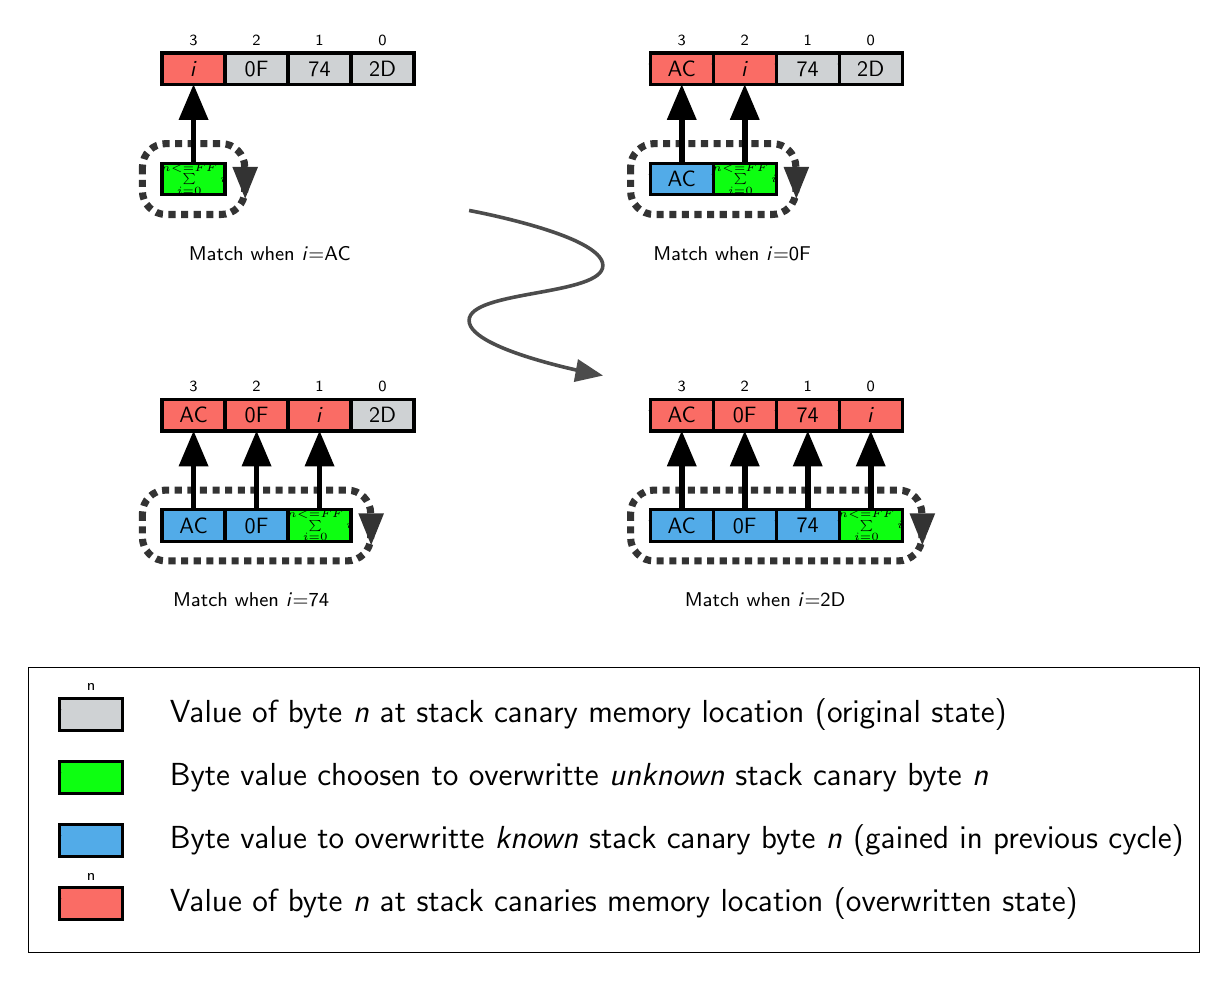
\begin{tikzpicture}[scale=1.0, every node/.style={scale=0.8},font=\sffamily,>=triangle 45]
    \tikzstyle{sum} = [draw, shape=circle, node distance=1.5cm, line width=1pt, minimum width=1.25em]
    \def\N{7}  % Number of Flip-Flops minus one
    
    \definecolor{c-stc-b}{HTML}{CFD2D4}
    \definecolor{c-try-byte}{HTML}{0DFF11}    
    \definecolor{c-try-byte-loop}{HTML}{000000}    
    \definecolor{c-fix-byte}{HTML}{52ABE8}        
    \definecolor{c-att-byte}{HTML}{F9473E}
    \definecolor{c-s-line}{HTML}{000000}
    \definecolor{c-leg-rect}{HTML}{FFF200}
    
    
%    stcan b3
%	\fontsize{7mm}{5.5cm}\selectfont
    \node [shape=dff, fill=c-att-byte!80] (rc-stcan-b3-3) at ($ 1.0*(4,0) $) {\textit{i}};
    \node [shape=dff, fill=c-stc-b, right=0mm of rc-stcan-b3-3.east, draw] (rc-stcan-b3-2) {0F};
    \node [shape=dff, fill=c-stc-b, right=0mm of rc-stcan-b3-2.east, draw] (rc-stcan-b3-1) {74};
    \node [shape=dff, fill=c-stc-b, right=0mm of rc-stcan-b3-1.east, draw] (rc-stcan-b3-0) {2D};
    \node[above=0mm of rc-stcan-b3-3.north] (lentp) {\scriptsize  3};                
    \node[above=0mm of rc-stcan-b3-2.north] (lentp) {\scriptsize  2};                    
    \node[above=0mm of rc-stcan-b3-1.north] (lentp) {\scriptsize  1};                    
    \node[above=0mm of rc-stcan-b3-0.north] (lentp) {\scriptsize  0};    
    \node [shape=dff, fill=c-try-byte, below=1cm of rc-stcan-b3-3.south, draw] (try-b3-3) {}; 
    \begingroup\makeatletter\def\f@size{5}\check@mathfonts
    \node (try-b3-3-inc) at (try-b3-3) {$\sum\limits_{i=0}^{n<=FF} i$};   
	\endgroup  
    
    \path (try-b3-3.west |- try-b3-3.north)+(-0.25,0.25) node (a) {};
    \path (try-b3-3.east |- try-b3-3.south)+(0.25,-0.25) node (b) {};
    \path [rounded corners=3mm, draw=c-try-byte-loop!80, line width=0.9mm, dotted] (a) rectangle (b);     
    \node[isosceles triangle, isosceles triangle apex angle=44,draw,
    inner sep=0pt,anchor=lower side,rotate=-90,draw=black, color=c-try-byte-loop!80,
    line width=1.3pt, minimum height=4mm, above right=1.5mm and 1.5mm of try-b3-3.east, fill=c-try-byte-loop!80] (try-byte-loop-b3) {};
    \node[below right=8mm and -7mm of try-byte-loop-b3.south] (lentp) {\small  Match when \textit{i}=AC};
    \draw [->, line width=2pt] (try-b3-3) -- (rc-stcan-b3-3);
                    
%%    stcan b2
    \node [shape=dff, fill=c-att-byte!80, right=3cm of rc-stcan-b3-0.east, draw] (rc-stcan-b2-3) {AC};
    \node [shape=dff, fill=c-att-byte!80, right=0mm of rc-stcan-b2-3.east, draw] (rc-stcan-b2-2) {\textit{i}};
    \node [shape=dff, fill=c-stc-b, right=0mm of rc-stcan-b2-2.east, draw] (rc-stcan-b2-1) {74};
    \node [shape=dff, fill=c-stc-b, right=0mm of rc-stcan-b2-1.east, draw] (rc-stcan-b2-0) {2D};            
    \node[above=0mm of rc-stcan-b2-3.north] (lentp) {\scriptsize  3};                
    \node[above=0mm of rc-stcan-b2-2.north] (lentp) {\scriptsize  2};                    
    \node[above=0mm of rc-stcan-b2-1.north] (lentp) {\scriptsize  1};                    
    \node[above=0mm of rc-stcan-b2-0.north] (lentp) {\scriptsize  0};                    
    \node [shape=dff, fill=c-fix-byte, below=1cm of rc-stcan-b2-3.south, draw] (try-b2-3) {AC};    
    \node [shape=dff, fill=c-try-byte, right=0mm of try-b2-3.east, draw] (try-b2-2) {};
    \begingroup\makeatletter\def\f@size{5}\check@mathfonts
    \node (try-b2-2-inc) at (try-b2-2) {$\sum\limits_{i=0}^{n<=FF} i$};   
    \endgroup          
    \path (try-b2-3.west |- try-b2-3.north)+(-0.25,0.25) node (a) {};
    \path (try-b2-2.east |- try-b2-2.south)+(0.25,-0.25) node (b) {};
    \path [rounded corners=3mm, draw=c-try-byte-loop!80, line width=0.9mm, dotted] (a) rectangle (b);     
    \node[isosceles triangle, isosceles triangle apex angle=44,draw,
    inner sep=0pt,anchor=lower side,rotate=-90,draw=black, color=c-try-byte-loop!80,
    line width=1.3pt, minimum height=4mm, above right=1.5mm and 1.5mm of try-b2-2.east, fill=c-try-byte-loop!80] (try-byte-loop-b2) {};
    \node[below right=8mm and -18mm of try-byte-loop-b2.south] (lentp) {\small  Match when \textit{i}=0F};
    \draw [->, line width=2pt] (try-b2-3) -- (rc-stcan-b2-3);
    \draw [->, line width=2pt] (try-b2-2) -- (rc-stcan-b2-2);    

%%    stcan b1
    \node [shape=dff, fill=c-att-byte!80, below=4cm of rc-stcan-b3-3.south, draw] (rc-stcan-b1-3) {AC};
    \node [shape=dff, fill=c-att-byte!80, right=0mm of rc-stcan-b1-3.east, draw] (rc-stcan-b1-2) {0F};
    \node [shape=dff, fill=c-att-byte!80, right=0mm of rc-stcan-b1-2.east, draw] (rc-stcan-b1-1) {\textit{i}};
    \node [shape=dff, fill=c-stc-b, right=0mm of rc-stcan-b1-1.east, draw] (rc-stcan-b1-0) {2D};            
    \node[above=0mm of rc-stcan-b1-3.north] (lentp) {\scriptsize  3};                
    \node[above=0mm of rc-stcan-b1-2.north] (lentp) {\scriptsize  2};                    
    \node[above=0mm of rc-stcan-b1-1.north] (lentp) {\scriptsize  1};                    
    \node[above=0mm of rc-stcan-b1-0.north] (lentp) {\scriptsize  0};        
    
    \node [shape=dff, fill=c-fix-byte, below=1cm of rc-stcan-b1-3.south, draw] (try-b1-3) {AC};    
    \node [shape=dff, fill=c-fix-byte, right=0mm of try-b1-3.east, draw] (try-b1-2) {0F};    
    \node [shape=dff, fill=c-try-byte, right=0mm of try-b1-2.east, draw] (try-b1-1) {};    
    \begingroup\makeatletter\def\f@size{5}\check@mathfonts
    \node (try-b1-1-inc) at (try-b1-1) {$\sum\limits_{i=0}^{n<=FF} i$};   
    \endgroup              
    \path (try-b1-3.west |- try-b1-3.north)+(-0.25,0.25) node (a) {};
    \path (try-b1-1.east |- try-b1-1.south)+(0.25,-0.25) node (b) {};
    \path [rounded corners=3mm, draw=c-try-byte-loop!80, line width=0.9mm, dotted] (a) rectangle (b);     
    \node[isosceles triangle, isosceles triangle apex angle=44,draw,
    inner sep=0pt,anchor=lower side,rotate=-90,draw=black, color=c-try-byte-loop!80,
    line width=1.3pt, minimum height=4mm, above right=1.5mm and 1.5mm of try-b1-1.east, fill=c-try-byte-loop!80] (try-byte-loop-b1) {};
    \node[below right=8mm and -25mm of try-byte-loop-b1.south] (lentp) {\small  Match when \textit{i}=74};
    \draw [->, line width=2pt] (try-b1-3) -- (rc-stcan-b1-3);
    \draw [->, line width=2pt] (try-b1-2) -- (rc-stcan-b1-2);        
    \draw [->, line width=2pt] (try-b1-1) -- (rc-stcan-b1-1);    
                
    
%%    stcan b0
    \node [shape=dff, fill=c-att-byte!80, right=3cm of rc-stcan-b1-0.east, draw] (rc-stcan-b0-3) {AC};
    \node [shape=dff, fill=c-att-byte!80, right=0mm of rc-stcan-b0-3.east, draw] (rc-stcan-b0-2) {0F};
    \node [shape=dff, fill=c-att-byte!80, right=0mm of rc-stcan-b0-2.east, draw] (rc-stcan-b0-1) {74};
    \node [shape=dff, fill=c-att-byte!80, right=0mm of rc-stcan-b0-1.east, draw] (rc-stcan-b0-0) {\textit{i}};            
    \node[above=0mm of rc-stcan-b0-3.north] (lentp) {\scriptsize  3};                
    \node[above=0mm of rc-stcan-b0-2.north] (lentp) {\scriptsize  2};                    
    \node[above=0mm of rc-stcan-b0-1.north] (lentp) {\scriptsize  1};                    
    \node[above=0mm of rc-stcan-b0-0.north] (lentp) {\scriptsize  0};                    
    \node [shape=dff, fill=c-fix-byte, below=1cm of rc-stcan-b0-3.south, draw] (try-b0-3) {AC};    
    \node [shape=dff, fill=c-fix-byte, right=0mm of try-b0-3.east, draw] (try-b0-2) {0F};    
    \node [shape=dff, fill=c-fix-byte, right=0mm of try-b0-2.east, draw] (try-b0-1) {74};        
    \node [shape=dff, fill=c-try-byte, right=0mm of try-b0-1.east, draw] (try-b0-0) {};   
    \begingroup\makeatletter\def\f@size{5}\check@mathfonts
    \node (try-b0-0-inc) at (try-b0-0) {$\sum\limits_{i=0}^{n<=FF} i$};   
    \endgroup              
    \path (try-b0-3.west |- try-b0-3.north)+(-0.25,0.25) node (a) {};
    \path (try-b0-0.east |- try-b0-0.south)+(0.25,-0.25) node (b) {};
    \path [rounded corners=3mm, draw=c-try-byte-loop!80, line width=0.9mm, dotted] (a) rectangle (b);     
    \node[isosceles triangle, isosceles triangle apex angle=44,draw,
    inner sep=0pt,anchor=lower side,rotate=-90,draw=black, color=c-try-byte-loop!80,
    line width=1.3pt, minimum height=4mm, above right=1.5mm and 1.5mm of try-b0-0.east, fill=c-try-byte-loop!80] (try-byte-loop-b0) {};
    \node[below right=8mm and -30mm of try-byte-loop-b0.south] (lentp) {\small  Match when \textit{i}=2D};
    \draw [->, line width=2pt] (try-b0-3) -- (rc-stcan-b0-3);
    \draw [->, line width=2pt] (try-b0-2) -- (rc-stcan-b0-2);        
    \draw [->, line width=2pt] (try-b0-1) -- (rc-stcan-b0-1);
    \draw [->, line width=2pt] (try-b0-0) -- (rc-stcan-b0-0);
    \node  (xxx) [below right=1.5cm and 1cm of rc-stcan-b3-0.south]{}; 
    \node  (yyy) [below right=0.5cm and 1.5cm of xxx]{}; 
    \node  (qqq) [below left=0.5cm and 1.5 cm of yyy]{}; 
    \node  (zzz) [below right=0.5cm and 1.5cm of qqq]{};     
    \draw [->, c-s-line!70, xshift=4cm, line width=1.3pt] plot [smooth, tension=1] coordinates { (xxx) (yyy) (qqq) (zzz)};
    
%    \begin{scope}[transform canvas={scale=0.8}]
    \begin{scope}[scale=0.8, every node/.style={scale=0.8},font=\sffamily,>=triangle 45]
    \tikzstyle{sum} = [draw, shape=circle, node distance=1.5cm, line width=1pt, minimum width=1.25em]
    \node [shape=dff, fill=c-stc-b, below left=8.0cm and 5mm of rc-stcan-b3-3.west, draw] (rc-leg-stc) {};
    \node[above=0mm of rc-leg-stc.north] (lentp) {\scriptsize  n};        
    \node[right=0.5cm of rc-leg-stc.east] (txt-leg-stc) {\Large{Value of byte \textit{n} at stack canary memory location (original state)}};        
    \node [shape=dff, fill=c-try-byte, below right=4mm and 0mm of rc-leg-stc.south west, draw] (rc-leg-try) {};
    %\node[above=0mm of rc-leg-try.north] (sdfdf) {\scriptsize  n};        
    \node[right=0.5cm of rc-leg-try] (txt-leg-try) {\Large{Byte value choosen to overwritte \textit{unknown} stack canary byte \textit{n}}};        
    \node [shape=dff, fill=c-fix-byte, below right=4mm and 0mm of rc-leg-try.south west, draw] (rc-leg-knw) {};
    %\node[above=0mm of rc-leg-knw.north] (sdfdf) {\scriptsize  n};    
    \node[right=0.5cm of rc-leg-knw] (txt-leg-knw) {\Large{Byte value to overwritte \textit{known} stack canary byte \textit{n} (gained in previous cycle)}};        
    \node [shape=dff, fill=c-att-byte!80, below right=4mm and 0mm of rc-leg-knw.south west, draw] (rc-leg-att) {};
    \node[above=0mm of rc-leg-att.north] (sdfdf) {\scriptsize  n};        
    \node[right=0.5cm of rc-leg-att] (txt-leg-att) {\Large{Value of byte \textit{n} at stack canaries memory location (overwritten state)}};    
    
    \draw[black] ([xshift=-5mm, yshift=5mm ]rc-leg-stc.north west) rectangle ([xshift=18mm, yshift=-4mm]txt-leg-att.south east);
    
    \end{scope}    
    \end{tikzpicture}
	\caption{Byte for Byte attack} \label{fig:byte-for-byte}
\end{figure}



% ... and so on until
\chapter{The Final Chapter}
\label{cha:n}
\lipsum[79]

\section{The First Topic of this Chapter}
\subsection{Item 1}
\subsubsection{Sub-item 1}
\lipsum[80]

\subsubsection{Sub-item 2}
\lipsum[81]

\subsection{Item 2}
\lipsum[82]

\section{The Second Topic}
\lipsum[83-85]

\section{Conclusion}
\lipsum[86-88]

%%% Local Variables: 
%%% mode: latex
%%% TeX-master: "thesis"
%%% End: 

\chapter{Notes}
\label{cha:notes}

\section{Experimental Setup/Analysis}
Processing/Algorithm is well known, 

\section{NIST}


%%% Local Variables: 
%%% mode: latex
%%% TeX-master: "thesis"
%%% End: 


\section{Discussion}

'It has been shown that the overlapping template matching test included in the NIST randomness test suite uses the inaccurate occurrence probabilities PI of the template.'
\cite{hamano2007correction,chen2016templates}. \cite{chen2016templates} proposal of approach, identification of relevant templates by correlation check. If templates B \&  B' have low correlation
both are selected for a test. If the correlation is high just one of both is chosen, as it is assumed to represent the discarded to the greatest extent. This approach reduces the amount of templates significantly (50 \%) \cite{chen2016templates}.

------------

BIOS serial number is ignored

------------

cycles and jiffies may provide more entropy at ungleichermassiger CPU load

------------

interrupt analyse ocnfidence lvele 0.05 ausreichend ?

------------

\chapter{Conclusion}
\label{cha:conclusion}
The final chapter contains the overall conclusion. It also contains
suggestions for future work and industrial applications.

\lipsum[1-7]

%%% Local Variables: 
%%% mode: latex
%%% TeX-master: "thesis"
%%% End: 


% If you have appendices:
\appendixpage*          % if wanted
\appendix
\chapter{The First Appendix}
\label{app:A}
Appendices hold useful data which is not essential to understand the work
done in the master's thesis. An example is a (program) source.
An appendix can also have sections as well as figures and references\cite{h2g2}.

\section{More Lorem}
\lipsum[50]

\subsection{Lorem 15--17}
\lipsum[15-17]

\subsection{Lorem 18--19}
\lipsum[18-19]

\section{Lorem 51}
\lipsum[51]

%%% Local Variables: 
%%% mode: latex
%%% TeX-master: "thesis"
%%% End: 

% ... and so on until
\chapter{The Last Appendix}
\label{app:n}
Appendices are numbered with letters, but the sections and subsections use
arabic numerals, as can be seen below.

\section{Lorem 20-24}
\lipsum[20-24]

\section{Lorem 25-27}
\lipsum[25-27]

%%% Local Variables: 
%%% mode: latex
%%% TeX-master: "thesis"
%%% End: 


\backmatter
% The bibliography comes after the appendices.
% You can replace the standard "abbrv" bibliography style by another one.
\bibliographystyle{abbrv}
\bibliography{references}

\end{document}

%%% Local Variables: 
%%% mode: latex
%%% TeX-master: t
%%% End: 
